%!TEX root = ../thesis.tex
\chapter{绪论}

%%%%%%%%%%%%%%%%%%%%%%%%%%%%%%%%%%%%%%%%%%%%%%%%%%%%%%%%%%%%%%%%%%%
\section{选题背景和研究意义}

我国城市轨道交通建设正处于飞速发展的阶段,截至2017年12月31日,中国内地累计有34个城市建成投运城轨线路5021.7公里;在“十二五”期间,累积新投运线路2019km,完成累积投资12289亿元,未来投资将持续增长,如图~\ref{fig:城市轨道交通投资额}~所示。建设规模居世界之首(轨道城市,\citeyear{轨道2017})。同时,国家发改委、住建部发布了首部国家级市政基础设施规划(住房和城乡建设部,\citeyear{住房和城乡建设部}),中国所倡导的“一带一路”宏伟计划,势必将轨道交通的建设推向一个新的高潮。随着轨道交通的建成与投入运营,作为城市的交通命脉,在100年的设计寿命期内,修筑于岩土介质的盾构隧道结构健康服役性能对于城市正常运转至关重要,越来越受到社会的广泛关注。例如北京、上海、广州等超大城市,一旦城市轨道交通的任一节点出现问题,将波及整个地铁网络,阻碍几百万人的出行,进而造成城市交通系统的瘫痪和恶劣的社会影响。

\begin{figure}[!h]
	\centering
	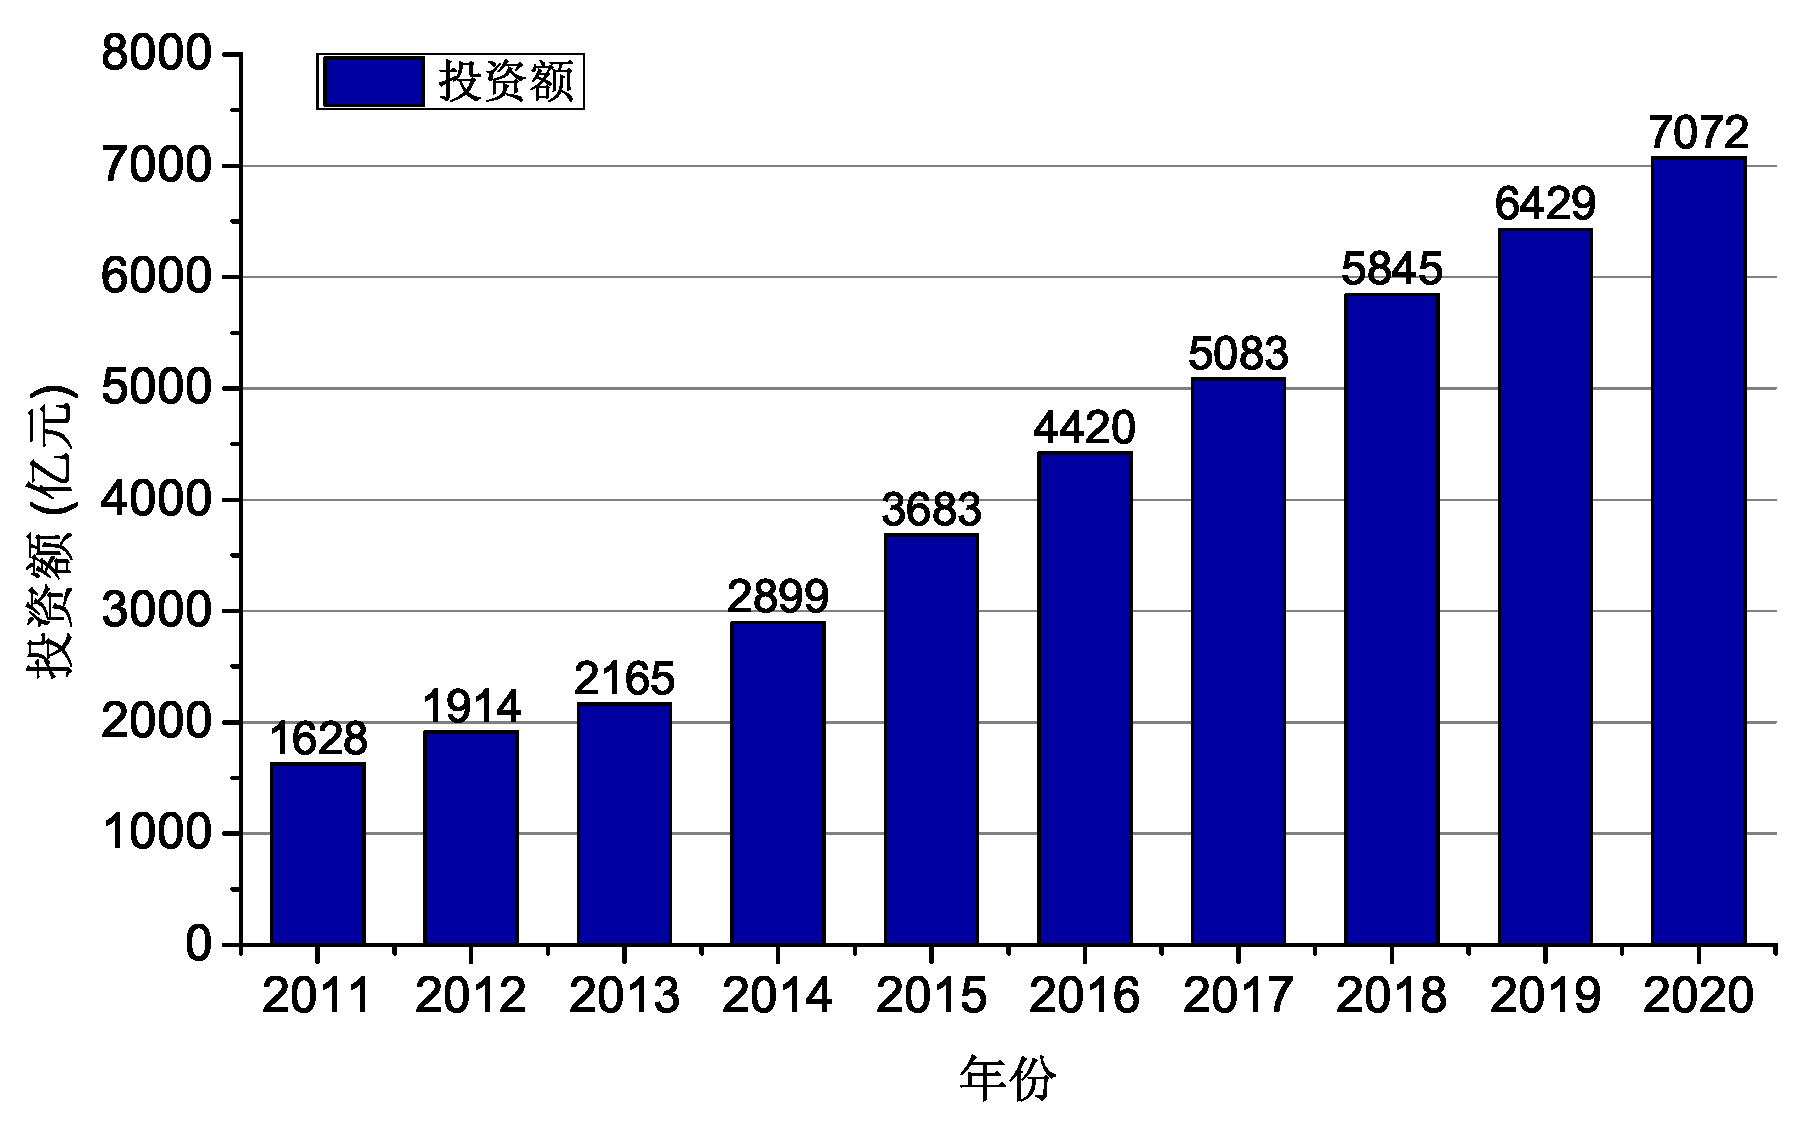
\includegraphics[width=0.7\textwidth]{chap1/investment.eps}
	\caption{中国城市轨道交通投资额}
	\label{fig:城市轨道交通投资额}
\end{figure}

我国城市轨道交通建设发展快但历史短,人们对结构健康服役问题的严重性重视程度不够。作为重大地下工程的城市轨道交通盾构隧道,所处岩土条件复杂、周边环境敏感、列车运行密度极高、使用条件苛刻,结构自身在多因素长期作用下性能不断劣化,一旦损坏不易或不可更换,并将会诱发地下工程灾害,因而对城市轨道交通盾构隧道健康服役提出了极高的要求。目前运营中的城市轨道交通健康服役问题已开始显露。

上世纪70年代建成的香港地铁部分隧道,在90年代就发现内排钢筋严重锈蚀,导致混凝土保护层的剥落,影响到正常使用。2001年5月22日,台北地铁淡水线士林站附近道床发生裂缝,地铁被迫减速,并改为手动驾驶,10万旅客上班受阻。北京地铁第一期工程1971年投入运营数年后,发现严重的杂散电流,已造成主体结构钢筋腐蚀,隧道内水管腐蚀穿孔。2006年8月19日,上海轨道交通2号线河南路-陆家嘴站越江隧道泵站由于振动与结构渗漏水的耦合叠加作用发生涌水冒浆险情,造成停运数小时。2009年12月22日,上海轨道交通1号线由于隧道结构顶部碳纤维脱落造成陕西南路至人民广场区间突发供电触网跳闸故障,造成该区列车停驶,16万人受困于地铁内、数百万人出行受阻,为建国以来城市轨道交通发生的最大事故。 

国外同样,2017年美国土木工程师协会(ASCE,\citeyear{ASCE2017})评价美国土木基础设施的平均等级为D+,估计需要花费20000亿美元才能够挽救这种长期忽视的问题。1999年10月9日,日本山阳城际新干线Kitakyushu隧道发生混凝土掉落击中电网事故,造成多趟列车取消,62000人因此出行受阻,事故调查显示原因是由于混凝土施工过程中存在缺陷,在渗漏、温度变化、列车振动等长期作用下导致裂隙不断发展所致。列宁格勒地铁1号线“森林”车站到“英勇广场”车站区间 1975 年投入运营。1994年隧道(通过钢板隔水层上的卸压排水管)经常间歇性涌水涌砂,1995年12月3日夜,下线隧道大量涌水,上线隧道急剧下沉,1995年12月4日,隧道运营终止。

上述事故表明,城市轨道交通地下结构在服役环境不断变化、材料劣化等内外因素共同作用下,其受力状态会发生变化,性能逐步退化,加之我国轨道交通建设速度迅猛,其结构施工质量难免存在一定程度的缺陷,因而城市轨道交通盾构隧道健康服役面临的问题日益突出。

综上所述,本文的研究意义体现在以下三个方面:(1)盾构隧道服役性能评估与分析有助于延长隧道的使用寿命。在隧道投入运营后,病害的出现势必缩短隧道使用寿命,适时合理的维修有助于延长隧道寿命。通过隧道结构服役性能理论研究,可以指导隧道维修时机,掌握隧道服役性能状况,制定科学的维修加固措施,延长隧道的结构劣化。

(2)盾构隧道服役性能评估与分析有助于提升城市轨道交通的社会形象。隧道作为轨道交通线路的重要一环,其健康安全是整条线路通畅运行的基础,一旦出现安全事故或列车停运,其社会负面影响将是难以估量的,严重时会影响到社会的稳定。因此全面掌握隧道服役性能状态,将安全隐患消灭在萌芽状态,保证线路的安全畅通。

(3)盾构隧道服役性能评估与分析有助于降低城市轨道交通养护维护成本。目前各国的土建结构维护费改建费增加迅速,维护费用成为财政的巨大负担。由于目前盾构隧道结构健康评估理论的不成熟,导出盲目维修、过度维修的现象,不但使得隧道病害未能得到有效治理,也造成巨大的经济浪费。因此对隧道服役性能的研究,可以以最少的资金投入达到最优的治理效果,具有重大的经济效益。

%%%%%%%%%%%%%%%%%%%%%%%%%%%%%%%%%%%%%%%%%%%%%%%%%%%%%%%%%%%%%%%%%%%
\section{国内外研究现状}
%+++++++++++++++++++++++++++++++++++++++++++++++++++++++++++++++++%
\subsection{盾构隧道服役性能评估进展}

目前隧道的服役性能评估方法大致可以分为三种:(1)基于隧道不同单项指标的劣化程度对隧道结构进行评估,在实际工作中最为常用,各国的隧道养护维护规范、手册均给出不同指标的评判标准;(2)基于历史数据建立数学模型对隧道结构进行综合性评估,如专家打分、决策树、概率论、层次分析法、模糊综合等;(3)基于数值模拟分析的评估方法,通过建立精细化数值模型,分析评估指标的评判标准。

\subsubsection{基于单项指标的评估方法}

日本《公路隧道维持管理便览》(日本公路协会,\citeyear{日本公路协会2000公路隧道维持管理便览})主要从隧道病害的发展和掉落的危险性和紧急程度来划分,根据隧道病害的严重性,从外力、材料劣化以及漏水等三个方面考虑,将评估指标划分为3A、2A、A、B四个等级,给出了衬砌变形、沉降、裂缝、剥落、漏水、湧砂、混凝土强度降低、钢筋锈蚀等指标的评判标准。

美国《公路和铁路交通隧道检查手册》(FHWA,\citeyear{FHWA2005Highway})给出隧道病害检测的一般流程,将隧道病害分为轻度、中度和严重三个等级,并规定了病害定量或者定性的评估标准。同时该手册建立了隧道结构的状态的状态分级标准,总共分为0到9十个级别,但手册只是定性地给出这十个等级的评定标准,并未给出具体的、定量的评价方法。

我国《地铁设计规范》(GB50157,\citeyear{GB501572013})对各类隧道病害指标作了规定,如建议衬砌环的直径变形控制在4-6\%衬砌直径以内;地下车站、连接通道和机电设备集中区段的防水等级应为一级,不允许渗水,结构表面无湿渍,区间隧道及连接通道等附属隧道机构防水等级应为二级,顶部不允许滴漏,其他不允许漏水,结构表面可有少量湿渍;衬砌管片的接缝张开量控制在1-2mm以内等。该规范并未对隧道状态评估进行规定。

我国《盾构法隧道结构服役性能鉴定规范》(DG/TJ08-2123-2013,\citeyear{DGTJ0821232013})根据设计规定、使用时间、使用条件和使用状况,进行结构服役性能鉴定。将隧道结构服役性能等级分级为正常、退化、劣化、恶化、危险五个等级,如表~\ref{tab:服役状态等级分级标准}~所示。将隧道结构服役状态鉴定分为五个层次,分别为隧道结构使用环境、构件服役状态等级评定、结构连接服役状态等级评定、结构区段服役状态等级评定和隧道整体服役状态等级评定,每一个层次的评定根据上一个层次评定结果所占比例决定。

\begin{table}[htbp]
  \centering
  \caption{盾构隧道服役状态等级分级标准}
    \begin{tabular}{?c"c"m{19.065em}"c?}
    \thickhline
    分级    & 服役状态  & \multicolumn{1}{c"}{分级定义} & 图示色彩 \bigstrut\\
    \thinhline
    i     & 正常    & 结构区段中的构件无安全隐患、无显著变形、无渗漏 & 绿色 \bigstrut\\
    \thinhline
    ii    & 退化    & 结构区段中部分构件耐久性退化,个别构件变形较大或结构连接处渗漏,但构件无安全隐患。 & 蓝色 \bigstrut\\
    \thinhline
    iii   & 劣化    & 结构区段中多数构件的耐久性劣化,整体变形较大或部分结构连接渗漏,但构件无安全隐患。 & 黄色 \bigstrut\\
    \thinhline
    iv    & 恶化    & 结构区段中整体变形较大 或多处结构连接明显渗漏,但无安全隐患。 & 橙色 \bigstrut\\
    \thinhline
    v     & 危险    & 结构区段中构件安全性不足、或结构区段变形过大或结构连接出现线流、漏泥沙。 & 红色 \bigstrut\\
    \thickhline
    \end{tabular}%
  \label{tab:服役状态等级分级标准}%
\end{table}%

\subsubsection{基于数学模型的评估方法}

吴江滨(\citeyear{吴江滨2004铁路运营隧道衬砌状态评估体系的建立及工程应用研究})在收集100余座铁路运营隧道数据基础上,提出隧道衬砌状态的评价体系,各个评价指标的评估标准根据应力集中系数给出,采用层次分析模型对隧道进行评估。但由于评价指标仅仅考虑了衬砌厚度和衬砌背后接触情况,评价指标过少,该评价体系未能很好反映隧道真实状态。

罗鑫(\citeyear{罗鑫2008公路隧道健康状态评估方法及系统研究})根据综合评估指标遴选原则和层次分析法原理,确定并建立了公路隧道结构健康状况综合评估体系,给出了不同评估指标的定量评定标准。采用乘积标度发确定指标的标度权重,再根据指标权重和样本数据,采用人工神经网络和模糊理论确定准则层指标权重,给出了隧道健康状态的模糊综合评价模型。

刘涛(\citeyear{刘涛2008既有盾构隧道结构性能评价研究})研究了现有城市盾构隧道的评估体系构成,和相应的评估工作流程,认为盾构隧道结构服役性能应该包含结构的安全性和耐久性,将评估指标分为整体的性能评估指标、安全性能的评估指标和耐久性的评估指标。并提出盾构隧道衬砌耐久性退化模型,基于Bayesian条件概率对耐久性模型进行修正,采用可靠度理论和Markov链方法对隧道结构的服役性能进行评价。

唐亮(\citeyear{唐亮2008隧道病害调查分析及衬砌结构的风险分析与控制研究})在分析隧道衬砌的主要破坏形式和影响结构安全性的风险因素基础上,设计了隧道风险的评价和接受准则,并根据故障树理论,建立隧道的衬砌结构故障树风险分析方法,对各种基本病害事件发生的概率,计算结构劣化的概率。在此之上,通过事件发生概率,提出可靠度理论的结构失效概率计算方法,辅以蒙特卡罗和有限元分析对隧道失效概率进行分析。

杨彤瑶等(\citeyear{杨彤瑶2013基于改进主元分析方法的隧道应变实时监测预警系统})针对隧道结构的实时监测异常数据分析,提出改进的主成分分析方法,即将原始数据流空间的变化趋势映射到对应的特征向量空间内,求解稳态特征向量,以瞬时特征向量和稳态特征向量关系,作为判据来对同步多维数据流进行异常变化诊断。在此基础上开发隧道实时监测预警系统,根据实测结果,该方法可以实时准确地反映隧道监测数据的异常变化。

李明等(\citeyear{李明2015基于功效系数法的隧道结构健康监测系统预警研究})引入功效系数法对隧道健康监测中的传感器监测数据的进行加权综合,实现监测数据的实时预警和评价。结合隧道结构健康监测系统特点,提出利用同一时刻所有传感器监测数据来确定结构预警指标体系,解决功效系数法中指标体系选取困难的问题。

Nývlt等(\citeyear{N2011Probabilistic})借鉴航天航空行业的风险分析概念,提出适合在隧道工程领域的风险分析方法,并结合决策树、可靠度理论、最优化方程等方法,建立满足安全风险级别下的成本最优化计算方法,该方法在实际工程应用中能指导养护维护决策,图~\ref{fig:隧道风险评估决策树}~为盾构隧道风险评估的决策树图。

\begin{figure}[!h]
	\centering
	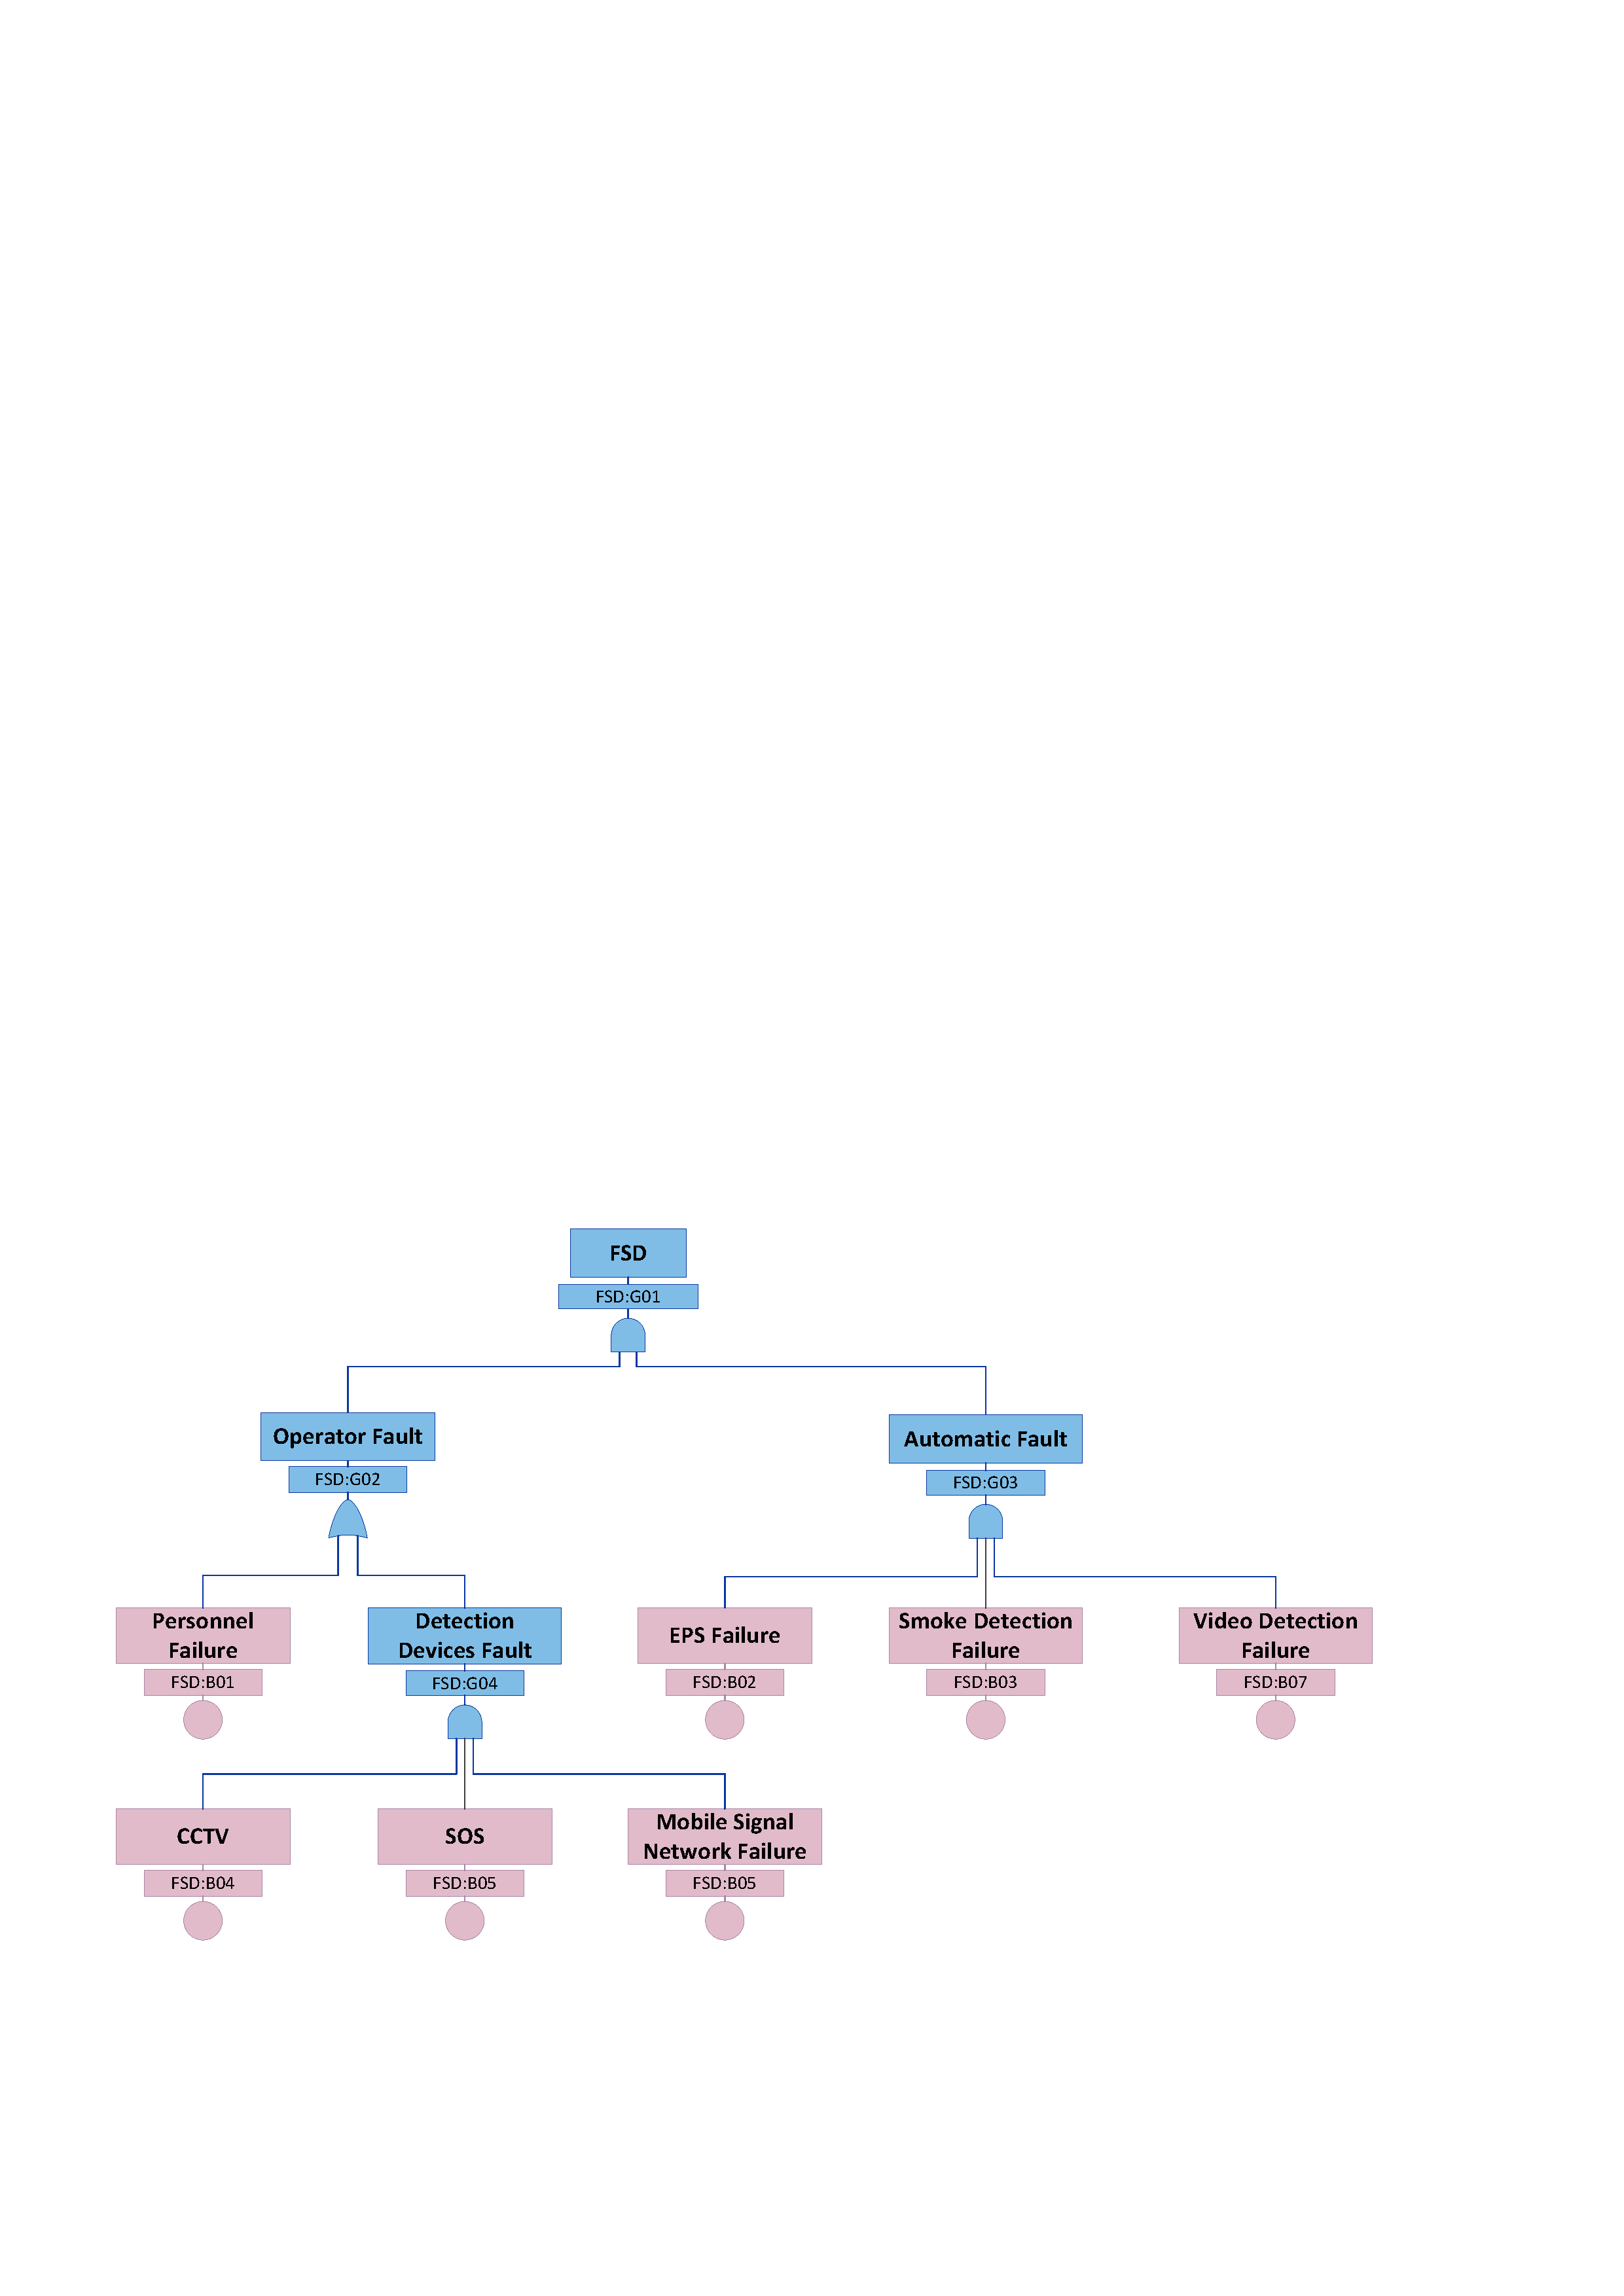
\includegraphics[width=1.0\textwidth]{chap1/nyvlt-faulttree.pdf}
	\caption{隧道风险评估决策树}
	\label{fig:隧道风险评估决策树}
\end{figure}

Yuan等(\citeyear{Yuan2012Assessment})为了量化隧道衬砌的结构性能,根据极限状态设计将其分为正常、退化、劣化、恶化、危险五个级别。结构的服役状态包括运营状态和结构状态。其中,运行状态指隧道所处环境条件环境恶劣程度。结构状态指标包括外观性、密封性、完整性、刚性和稳定性。提出了隧道结构服役状态评估的框架,依据运行状态指标和结构指标值与标准值的比较得出其所处的服役状态级别。

Zhang等(\citeyear{Zhang2014Fuzzy})采用模糊分析层次和综合评估模型,合并多个传感器的不同类型的数据,将其映射为盾构隧道的健康评分。选择分段隶属函数,并引入指数量表表征不同权重集。定义模糊运算符号,用于监测因子的模糊综合评估指标。

\subsubsection{基于力学模型的评估方法}

Cavalaro等(\citeyear{Cavalaro2011Structural})研究了施工期盾构隧道衬砌裂缝形成的主要机理,最常见的裂缝是由衬砌之间接触不均匀导致支撑受力不一致而产生的。通过建立不同的有限元模型并对比其分析结果,得出衬砌的接触不均匀直接影响了衬砌的极限承载力。

Naggar和Hinchberger(\citeyear{Naggar2012Approximate})采用数值分析方法,模拟完好的和劣化后的混凝土衬砌力学特性。使用非线性有限元模型模拟混凝土退化,并考虑了土体和混凝土的相互作用和非线性应力应变响应,用于评估劣化后的隧道衬砌的性能状态。

Li等(\citeyear{Li2015Experimental})研究了不同轴向应力水平下弯矩的纵向接缝张开的发展情况和极限状态中的纵向接缝张开,提出了一种渐进模型来预测接缝的力学行为。基于此模型,研究轴向应力水平,螺栓预紧力,混凝土分层深度和螺栓腐蚀深度对接缝力学性能的影响。

Li等(\citeyear{Li2015A})提出了纵缝接头张开的计算模型。模型包含接缝张开不同阶段的不同受力模式,考虑混凝土、螺栓和密封垫对张开量的影响。实验观测与计算分析得出纵缝张开过程可分为四个阶段:阶段一是一开始接缝未张开时,接头处混凝土全截面受压;阶段二接头处混凝土开始出现张开,螺栓拉力逐渐增大;阶段三为外侧边混凝土开始接触;阶段四则是螺栓屈服阶段,如图~\ref{fig:接缝张开与弯矩}~所示,此模型可用于指导盾构隧道衬砌的接缝张开评估。

\begin{figure}[!h]
	\centering
	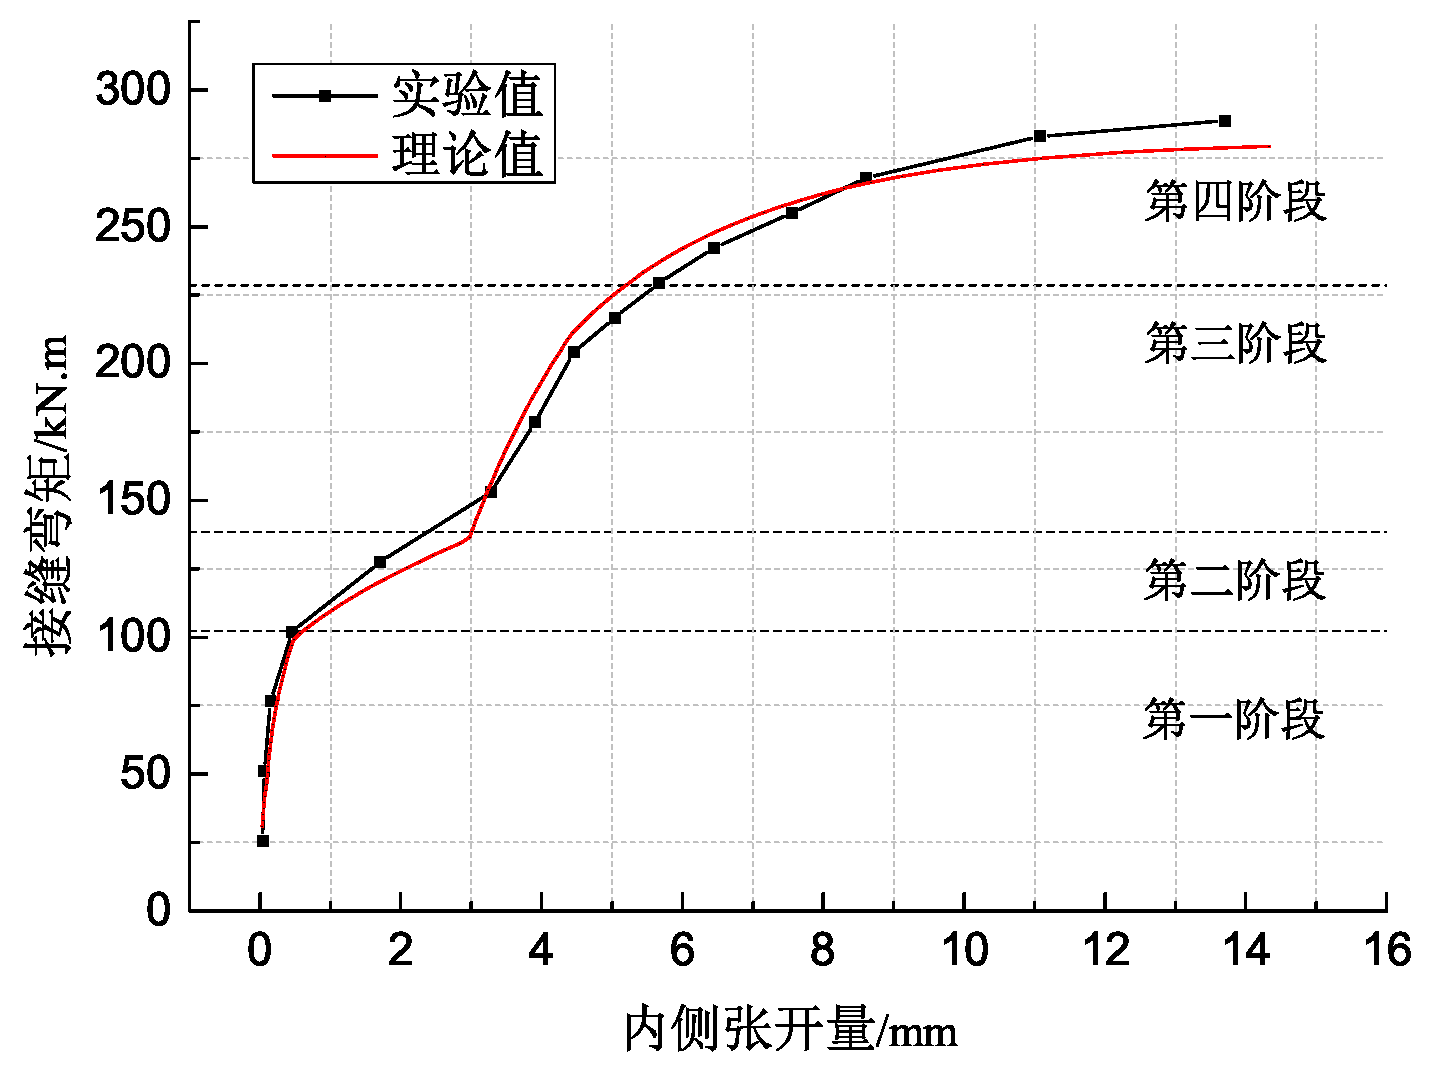
\includegraphics[width=0.7\textwidth]{chap1/joint-moment.eps}
	\caption{盾构隧道衬砌弯矩-接缝张开关系图}
	\label{fig:接缝张开与弯矩}
\end{figure}

袁勇等(\citeyear{袁勇2006运营越江隧道服役现状调查与检测评估})指出对于直径10~m的盾构隧道,隧道的纵向变形曲率半径小于40~km时,容易导致衬砌环向接头张开增大,引起渗漏。同时渗漏又导致隧道继续产生纵向不均匀变形,二者相互影响。并提出用于既有隧道结构损伤评估的宏观安全性模型和微观耐久性模型。

季倩倩(\citeyear{季倩倩2009带裂缝的盾构隧道衬砌力学模型研究})在盾构隧道的梁-弹簧计算模型中,采用弹簧单元模拟裂缝对衬砌结构的影响,建立了带裂缝的盾构隧道衬砌力学模型。分析结果指出裂缝的存在降低了衬砌的刚度,且降低程度与裂缝宽度和深度相关。

刘曙光(\citeyear{刘曙光2012盾构隧道混凝土管片的承载力退化模型})在现有钢筋混凝土正截面承载力计算方法基础上,考虑了锈蚀钢筋混凝土受弯构件的正截面承载力计算方法,提出盾构隧道衬砌的承载能力退化模型,模型有水平段的诱导期和下降段的劣化期组成,可用于盾构隧道混凝土管片的寿命评估。

王如路和张冬梅(\citeyear{王如路2013超载作用下软土盾构隧道横向变形机理及控制指标研究})采用数值模拟方法分析地面压载、土体侧向压力、土体抗力对盾构隧道收敛变形的影响,给出了收敛变形随压载的变化规律,得出收敛变形与衬砌受力、螺栓受力和接缝张开量的关系曲线,在实际工程中可根据隧道的直径测量量判断隧道的变形状态,为隧道的安全性评价提供指导。

丁文其等(\citeyear{丁文其2013基于地层})采用地层-结构法研究隧道初始地应力平衡、施工顺序、材料本构模型和接触关系等问题,分析不同因素对隧道沉降变形和接头相对变形的影响。

%+++++++++++++++++++++++++++++++++++++++++++++++++++++++++++++++++%
\subsection{盾构隧道服役性能预测进展}

针对盾构隧道结构出现的病害,现有的计算方法还很难全面模拟材料的真实特性、结构与环境的真实状态,因而难以准确评价结构服役性能和确定病害成因、发展趋势及其对服役性能的影响。目前主要有两类方法对盾构隧道服役性能进行预测:(1)考虑材料性能退化的影响,结合盾构隧道数值模型,分析服役性能的退化;(2)基于历史数据,建立数学模型,采用大量数据对模型参数进行估计训练。

\subsubsection{基于材料劣化的性能预测}

Marchand等(\citeyear{Marchand2002Theoretical})研究了弱硫酸根离子对混凝土耐久性的影响,分别试验了水灰比为0.45、0.65、0.75,CSA10和50类型水泥,硫酸盐浓度0-30~mmol/l的不同方案,得出混凝土在硫酸根离子溶液中的退化规律。

Liu等(\citeyear{Liu2014A})考虑早龄期混凝土各组分材料随机分布的影响,及由于水化反应造成的热力学性能时变性和体积变形,将宏观尺度划分为混凝土、砂浆、水泥浆三个不同尺度,对混凝土早龄期性能进行跨尺度研究。建立非线性粘弹性早龄期混凝土多尺度本构模型,并与时间耦合的本构关系。

李忠等(\citeyear{李忠2009氯离子侵蚀盾构隧道衬砌结构性能退化试验})对盾构隧道衬砌钢筋进行加速锈蚀实验,得到不同锈蚀程度的钢筋构件,再对锈蚀钢筋的承载力、变形和破坏特征等作相关测试,获取隧道衬砌结构在氯离子侵蚀下的性能退化规律。

张红光等(\citeyear{张红光2014开裂混凝土内氯离子扩散机理及数值模拟研究})研究得出混凝土结构在初始损伤和裂缝存在情况下,容易造成氯离子等侵蚀性介质在混凝土中快速扩散,通过实验观察和数值模拟,归纳氯离子在混凝土中的扩散系数表达式,为评价混凝土结构的耐久性提供依据。

\subsubsection{基于数学模型的性能预测}

在工程领域,退化模型包括马尔科夫链模型(Madanat等,\citeyear{Madanat1997Probabilistic})、时间序列模型(Prozzi,\citeyear{prozzi2001modeling})、泊松回归模型(Ching和Leu,\citeyear{ching2009bayesian})、灰色预测模型(Wang和Li,\citeyear{wang2011pavement})等,其中马尔科夫链和时间序列最为常用。

Carnahan等(\citeyear{camahan1987optimal})提出马尔科夫链是一种时间离散基于状态的退化模型,其基本假定包括:1)有限个状态;2)状态转移概率只依赖当前的状态;3)转移概率矩阵与时间无关。马尔科夫链模型的转移概率可通过期望值法来估计,但期望值法无法显式地表示影响因素对于状态的影响、考虑退化过程与时间的依赖性、表示连续的退化过程。

Madanat等(\citeyear{Madanat1997Probabilistic})分别采用了泊松回归模型、有序概率模型来估计马尔科夫链模型中的转移概率矩阵,解决了期望值法无法显式地表示影响因素对于状态的影响、考虑退化过程与时间的依赖性、表示连续的退化过程的问题,可以考虑导致状态变化的影响因素和时间因素。

DeStefano和Grivas(\citeyear{destefano1998method})提出了基于时间的模型以计算状态转移概率。Mishalani和Madanat(\citeyear{mishalani2002computation})提出了基于时间状态离散的随机持续时间模型,能够考虑时间、状态之间的依赖性,表征退化过程与影响因素之间的关系,并且用钢筋混凝土桥面板实例阐述了该方法的可行性。

Chu等(\citeyear{chu2005estimation})提出结构化时间序列模型,该模型可以解释采用不同数据采集方式获取的数据之间的不确定性,同时该模型也可辅助得出维护养护决策时的最优化方案,可以替代传统的马尔科夫链模型。

Chu等(\citeyear{chu2007estimation})采用自回归滑动平均时间序列模型(ARMA 模型)预估基础设施的性能变化,其能考虑状态空间的相互依赖性,预测样本空间外结构的性能变化趋势,也可作为马尔科夫链模型的一种替代方法。

曹净等(\citeyear{曹净2014基于})提出基于小波变换和粒子群优化的最小二乘支持向量机,结合自回归移动平均模型,预测基坑变形的时间序列数据。基于小波变化先将时间序列数据分解为趋势时间序列和随机时间序列两个子序列,分别采用支持向量机和自回归移动平均模型来预测两个子序列,最后再相叠加得到最终预测结果。

文明等(\citeyear{文明2015地铁车站施工过程中地表沉降的})针对时间序列模型的单一线性和忽略外部因素影响的问题,建立了非线性自回归神经网络时间序列模型,如图~\ref{fig:非线性自回归神经网络}~所示,该模型具有延迟单元和反馈结构,并且可以将外部因素作为外部输入,预测结果适应性更好、准确性更高。

\begin{figure}[!h]
	\centering
	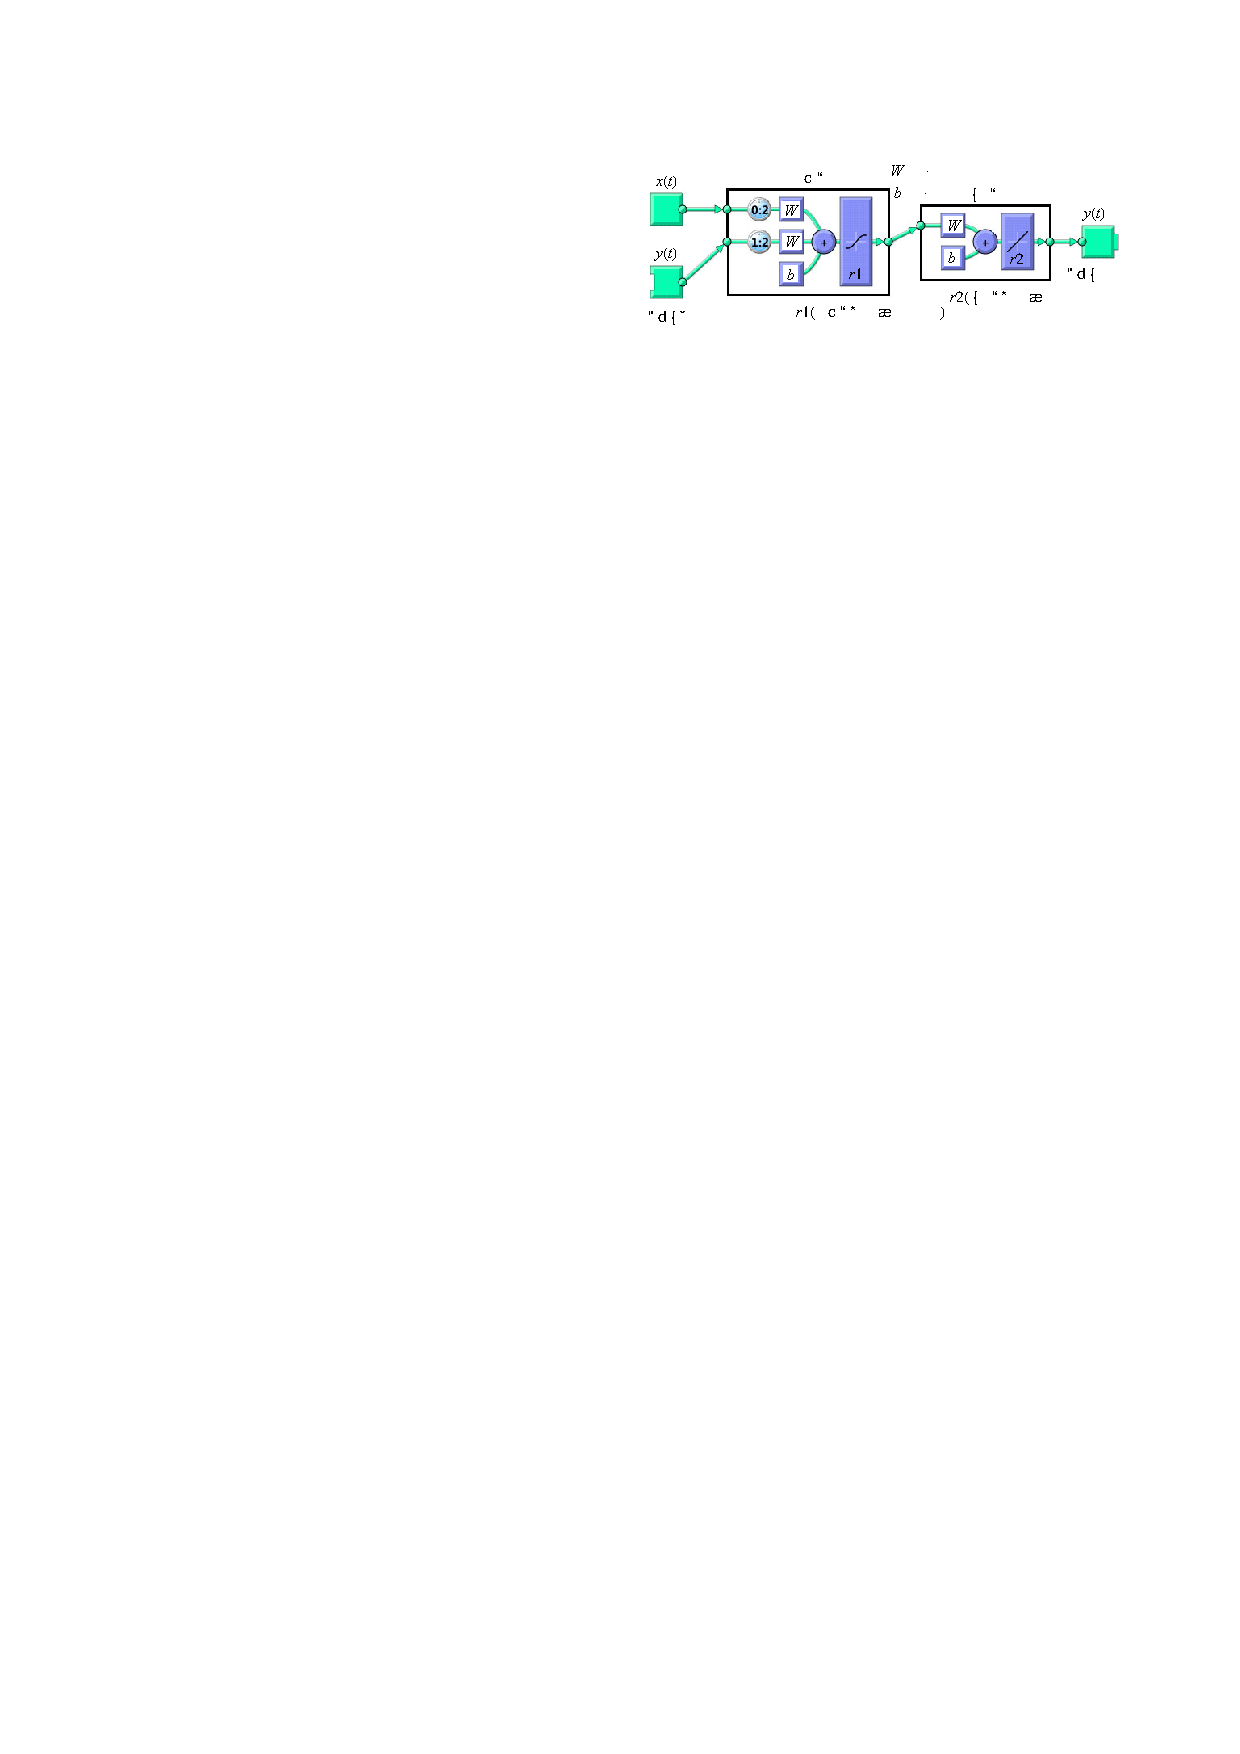
\includegraphics[width=0.7\textwidth]{chap1/NARXNN.pdf}
	\caption{非线性自回归神经网络时间序列模型(文明等,\citeyear{文明2015地铁车站施工过程中地表沉降的})}
	\label{fig:非线性自回归神经网络}
\end{figure}

%+++++++++++++++++++++++++++++++++++++++++++++++++++++++++++++++++%
\subsection{盾构隧道服役性能服务进展}
\label{chap:service-intro}

随着信息技术的不断发展,数字化技术成为改革传统模式的重要手段,高效的盾构隧道服役性能评估与预测服务同样需借助数字化技术。在土木工程领域,常用的数字化技术包括三大类:(1)地理信息系统(GIS);(2)建筑信息模型系统(BIM);(3)综合性的智慧服务系统。

\subsubsection{基于地理信息系统的服务平台}

地理信息系统(Geographic Information System,GIS)是一门结合地理学、地图学、遥感、计算机等的综合性学科,目前在不同的领域得到广泛应用,主要用于输入、存储、查询、显示和分析地理数据的系统。早期在地下工程主要用于地质数据的存储,如Rosenbaum和Warren(\citeyear{rosenbaum1986creating})早在1972年就为伦敦的地质钻孔数据建立了地理数据库,可用于地下公路、铁路开挖时的周边环境评估。

Baffour和Abatan(\citeyear{baffour2002developing})结合探地雷达(GPR)、全球定位系统(GPS)和地理信息系统,开发了地下基础设施的数字化采集、处理、管理信息系统,该系统具备空间信息和属性信息的管理能力,为地下基础设施提供定位、分析等高效的功能。

Chang和Park(\citeyear{chang2004development})基于Web技术开发了钻孔数据和地层数据的GIS管理系统,在系统建立在钻孔和地层的数据标准和数据库标准之上,合计存储了超过10000个钻孔和首尔地层等数据,用户通过互联网可以方便地对这些数据进行检索、统计分析。

近年GIS的地理数据分析功能逐渐被重视,如Yoo和Kim(\citeyear{yoo2007tunneling})首先用人工神经网络(ANNs)预测一般隧道设计中的隧道性能预测,对于隧道工程现场,经校正有限元模型改进过的ANNs能根据稳定性和附近环境的影响得出隧道环境和性能的关系。并把ANNs植入到GIS,利用GIS的数据管理和可视化功能进行分析,如图~\ref{fig:集成GIS和ANN的隧道掘进性能概念}~所示,该平台的最大优势是加快了隧道性能的评估,从而缩短隧道设计的时间。

\begin{figure}[!h]
	\centering
	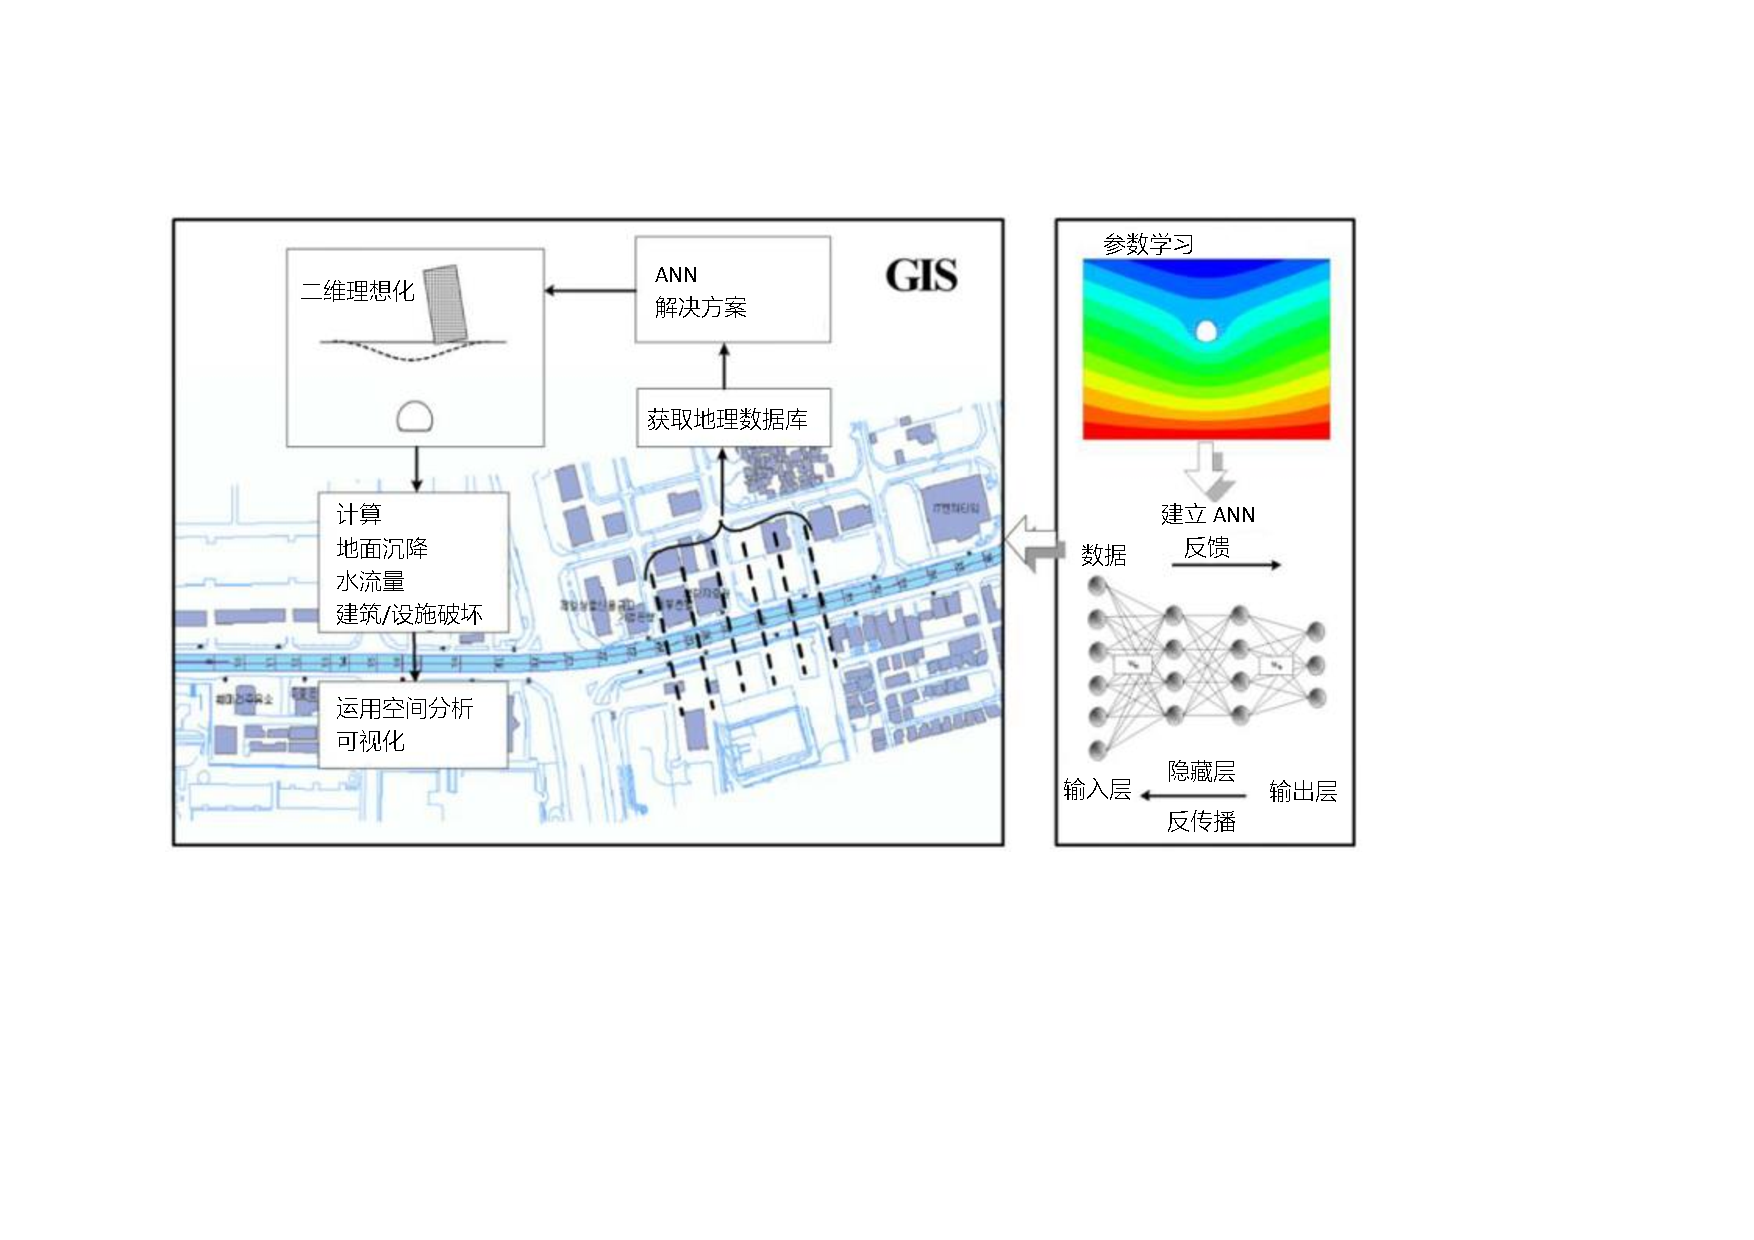
\includegraphics[width=0.9\textwidth]{chap1/ann-gis.pdf}
	\caption{集成GIS和ANN的隧道掘进性能概念(Yoo和Kim,\citeyear{yoo2007tunneling})}
	\label{fig:集成GIS和ANN的隧道掘进性能概念}
\end{figure}

Yuan等(\citeyear{yuan2012study})基于GIS数据管理,在GIS系统中实现了隧道开发对岩体变形和地表建筑物影响的分析功能,并建立数值模型分析由于开挖变形引起的地表建筑物的应力-应变关系曲线,该平台为隧道施工期间的防灾减灾提供了快速的评估依据。

Li和Zhu(\citeyear{li2013development})开发轨道交通数字化平台,以满足盾构隧道施工运营过程中数据管理、数据分析和可视化要求。根据已有工程数据标准,结合以往盾构隧道工程实例,提出轨道交通地下结构全生命周期数据标准和数据库设计,主要分为地质、结构和监测三部分。利用Web-GIS软件和Web Service技术开发基于互联网的数字化平台。

解福奇等(\citeyear{解福奇2009时态})建立了考虑时间的多维、动态GIS模型,可在该模型上对时态数据进行操作和处理,能实时反映时态数据属性的变化,且模型也提供了方便的数据库查询和检索功能,采用三维可视化技术将模型运用于隧道工程的数字化施工当中。

刘振平等(\citeyear{刘振平20173d})采用GRASS GIS、Python等建立了GIS和有限元模拟分析的开发框架,实现了网格剖分算法,改良3D GIS中的TIM模型,使其适合有限元模拟的地质切面的三角形网格,结合GIS的空间分析功能,得到GIS与有限元分析无缝结合的隧道地表沉降规律分析功能。

\subsubsection{基于建筑信息模型的服务平台}

建筑信息模型(Building Information Model,BIM)是以建筑工程项目的各类信息数据作为基础,建立三维建筑模型,通过数字仿真技术模拟建筑物所具有的所有真实信息。统一的建筑信息模型能让业主单位、设计单元、施工单位和监理单位等多个项目参与方,共享同一模型。目前BIM在土木工程中的应用包括三维可视化、成本造价、几何碰撞、施工仿真、能耗分析、养护维护等。

Motamedi和Hammad(\citeyear{motamedi2009lifecycle})认为BIM将成为工程全寿命周期中创建、共享、交换和管理信息的方法,当前RFID技术已经成为成熟的数据自动采集和信息存储技术,该技术可为BIM收集各类全寿命数据作为基础数据,讨论了BIM系统数据的存储和检索设计。

Zhang等(\citeyear{zhang2013building})将自动化安全规则检查集成在BIM模型中,开发了不同情况下的算法程序,可自动分析建筑模型和监测安全隐患,向用户建议预防措施。该系统可用于设计期的自动化危险识别和纠正,预防在施工期发生安全事故。

李德超和张瑞芝(\citeyear{李德超2012bim})将数字城市模型与BIM模型集成一体。数字城市模型主要利用GIS技术,以城市地理空间数据为基础,建立的城市数字信息模型,集成BIM可实现城市数字模型的资源共享,以及多领域对城市模型的协同作业。

于金勇和林敏(\citeyear{于金勇2013bim})将地铁设计电子图纸转换成BIM建筑、结构、机电模型,并整合在一起,利用BIM软件的碰撞分析得出碰撞点,对BIM模型进行重新设计消除碰撞点,优化了地铁安装工程的施工方案,避免了工程在验收阶段的返工误工现象出现。

王慧琛等(\citeyear{王慧琛2013bim})将BIM技术应用于地铁车站的设计期和施工期两个阶段,应用主要包括两个方面,一方面采用BIM技术对地铁车站工程建立全专业设施模型,分析各专业设备之间碰撞。另一方面也利用BIM模型对整体工程进行虚拟仿真及4D施工模拟。

BIM技术在应用过程中有三方面的挑战,包括标准层面、技术层面和管理层面,在BIM技术标准层面,最重要的内容即是建筑信息的数据交换标准。IFC(Industry Foundation Class)标准是国际通过的BIM数据标准,现有的IFC版本已经可以较好描述建筑工程的全寿命周期信息,对于地下基础设施领域的研究也已取得部分成果。

如Yabuki(\citeyear{yabuki2013development})在IFC标准基础上提出并改进了盾构隧道的数据模型IFC-ShieldTunnel。该数据模型在IFC框架内增加了盾构隧道特有的对象实体,如管片、防水材料等,并通过实际工程验证了模型的适用性。该研究团队还计划对该数据模型在盾构隧道施工进度和成本造价方面的扩展研究。IFC-ShieldTunnel基本确定了盾构隧道全寿命周期数据模型的框架体系。

Borrmann和Jubierre(\citeyear{borrmann2013multi})认为现有的IFC标准无法从多个详细程度对大型基础设施的信息进行描述,因此在Yabuki的盾构隧道信息模型基础上引入LoD和Refines实体,不同详细程度的信息对象进行定义。同时,为保持不同LoD间几何信息的连贯性,对不同LoD中几何对象的引用关系进行了研究。 

林浩(\citeyear{林浩2016基于})认为IFC-ShieldTunnel信息模型中定义的部分实体只是停留在语义状态,此外,在地质信息领域,IFC-ShieldTunnel 没有描述土工试验信息;在施工信息、监测信息和结构病害信息领域,IFC-ShieldTunnel也未见相关资料信息;故对IFC-ShieldTunnel进行扩展。

\subsubsection{综合性的智慧服务平台}

目前GIS和BIM系统应用于地下工程仍存在许多问题,如GIS对非地理数据只能将其作为地理数据的属性数据进行管理,而且GIS本身并没有规定数据标准,而是由用户自行定义,导致不同用户之间数据共享困难。BIM最初是针对地面建筑提出,逐渐扩展至土木工程的不同领域,但BIM没有提出完整的信息流概念,只是停留在对信息模型本身的管理,造成信息流通不通畅的问题。基于上述原因,许多学者提出开发了综合性的智慧服务平台。

朱合华和李晓军(\citeyear{朱合华2007数字地下空间与工程})系统提出了数字地下空间与工程的基本概念,其应提供开放的信息组织方法与信息发布机制,建立健全的数据标准与数据处理的方法,具备可视化手段。综合性的数字化地下空间与工程可以实现信息发布与共享,并对海量的工程数据进行动态管理,提供不同的数据可视化方式,从而提高工程管理效率。

李晓军等(\citeyear{李晓军2009盾构隧道数字化研究与应用})提出盾构隧道的数字化概念,即让复杂多变的地下工程变得更加透明,对工程全寿命周期数据的管理,最终辅助工程分析与智能决策。该系统采用客户端-服务器架构,将工程数据分为空间信息数据和属性信息数据两种,并对三维隧道和三维地层进行建模,实现工程可视化。

朱合华等(\citeyear{朱合华2015基础设施建养一体数字化技术})提出基础设施的建养一体数字化的概念,从基础设施建设和养护一体的角度考虑,结合工程、经济和管理的手段,以最优方式保障基础设施工程的安全。建养一体化的数字平台包括了数据采集、处理、表达、分析等功能,集成了采集技术、数据标准、可视化建模、空间分析和数字数值一体化分析等技术。

自从2008年IBM公司提出“智慧地球”的概念(IBM,\citeyear{IBM2008Wisdom}),“智慧化”一词成为新的研究热点。在土木领域,“智慧城市”的概念随之形成(巫细波和杨再高,\citeyear{巫细波2010智慧城市理念与未来城市发展}),结合物联网、云计算和大数据等信息技术,对城市中的基础设施赋予接入网络的能力,通过网络将城市基础设施联系在一起。智慧城市并不是单一技术的累加,而是“数字城市+物联网+云计算+大数据”(李德仁等,\citeyear{李德仁2013智慧城市的概念})。

英国剑桥大学于2011年成立智慧基础设施研究中心(Cambridge Centre for Smart Infrastructure and Construction,CSIC),此研究为响应英国政府颁发的英国基础设施建设计划(Treasury,\citeyear{treasury2011national}),收集掌握英国所有基础设施当前状态、制定合适的养护维护措施、降低维护成本和延长基础设施的使用寿命。CSIC(\citeyear{CSIC2011Cambridge})采用了无线传感器等监测手段,实现对基础设施的可持续发展的目标。

朱合华等(\citeyear{朱合华2018智慧基础设施})于2013年提出基础设施智慧服务系统(infrastructure Smart Service System,iS3)的概念,从信息流的角度,实现基础设施的智慧化管理。iS3系统包括数据的采集、处理、表达、分析和服务决策等五个方面,如图~\ref{fig:iS3概念图}~所示,并兼容GIS系统与BIM系统。

\begin{figure}[!h]
	\centering
	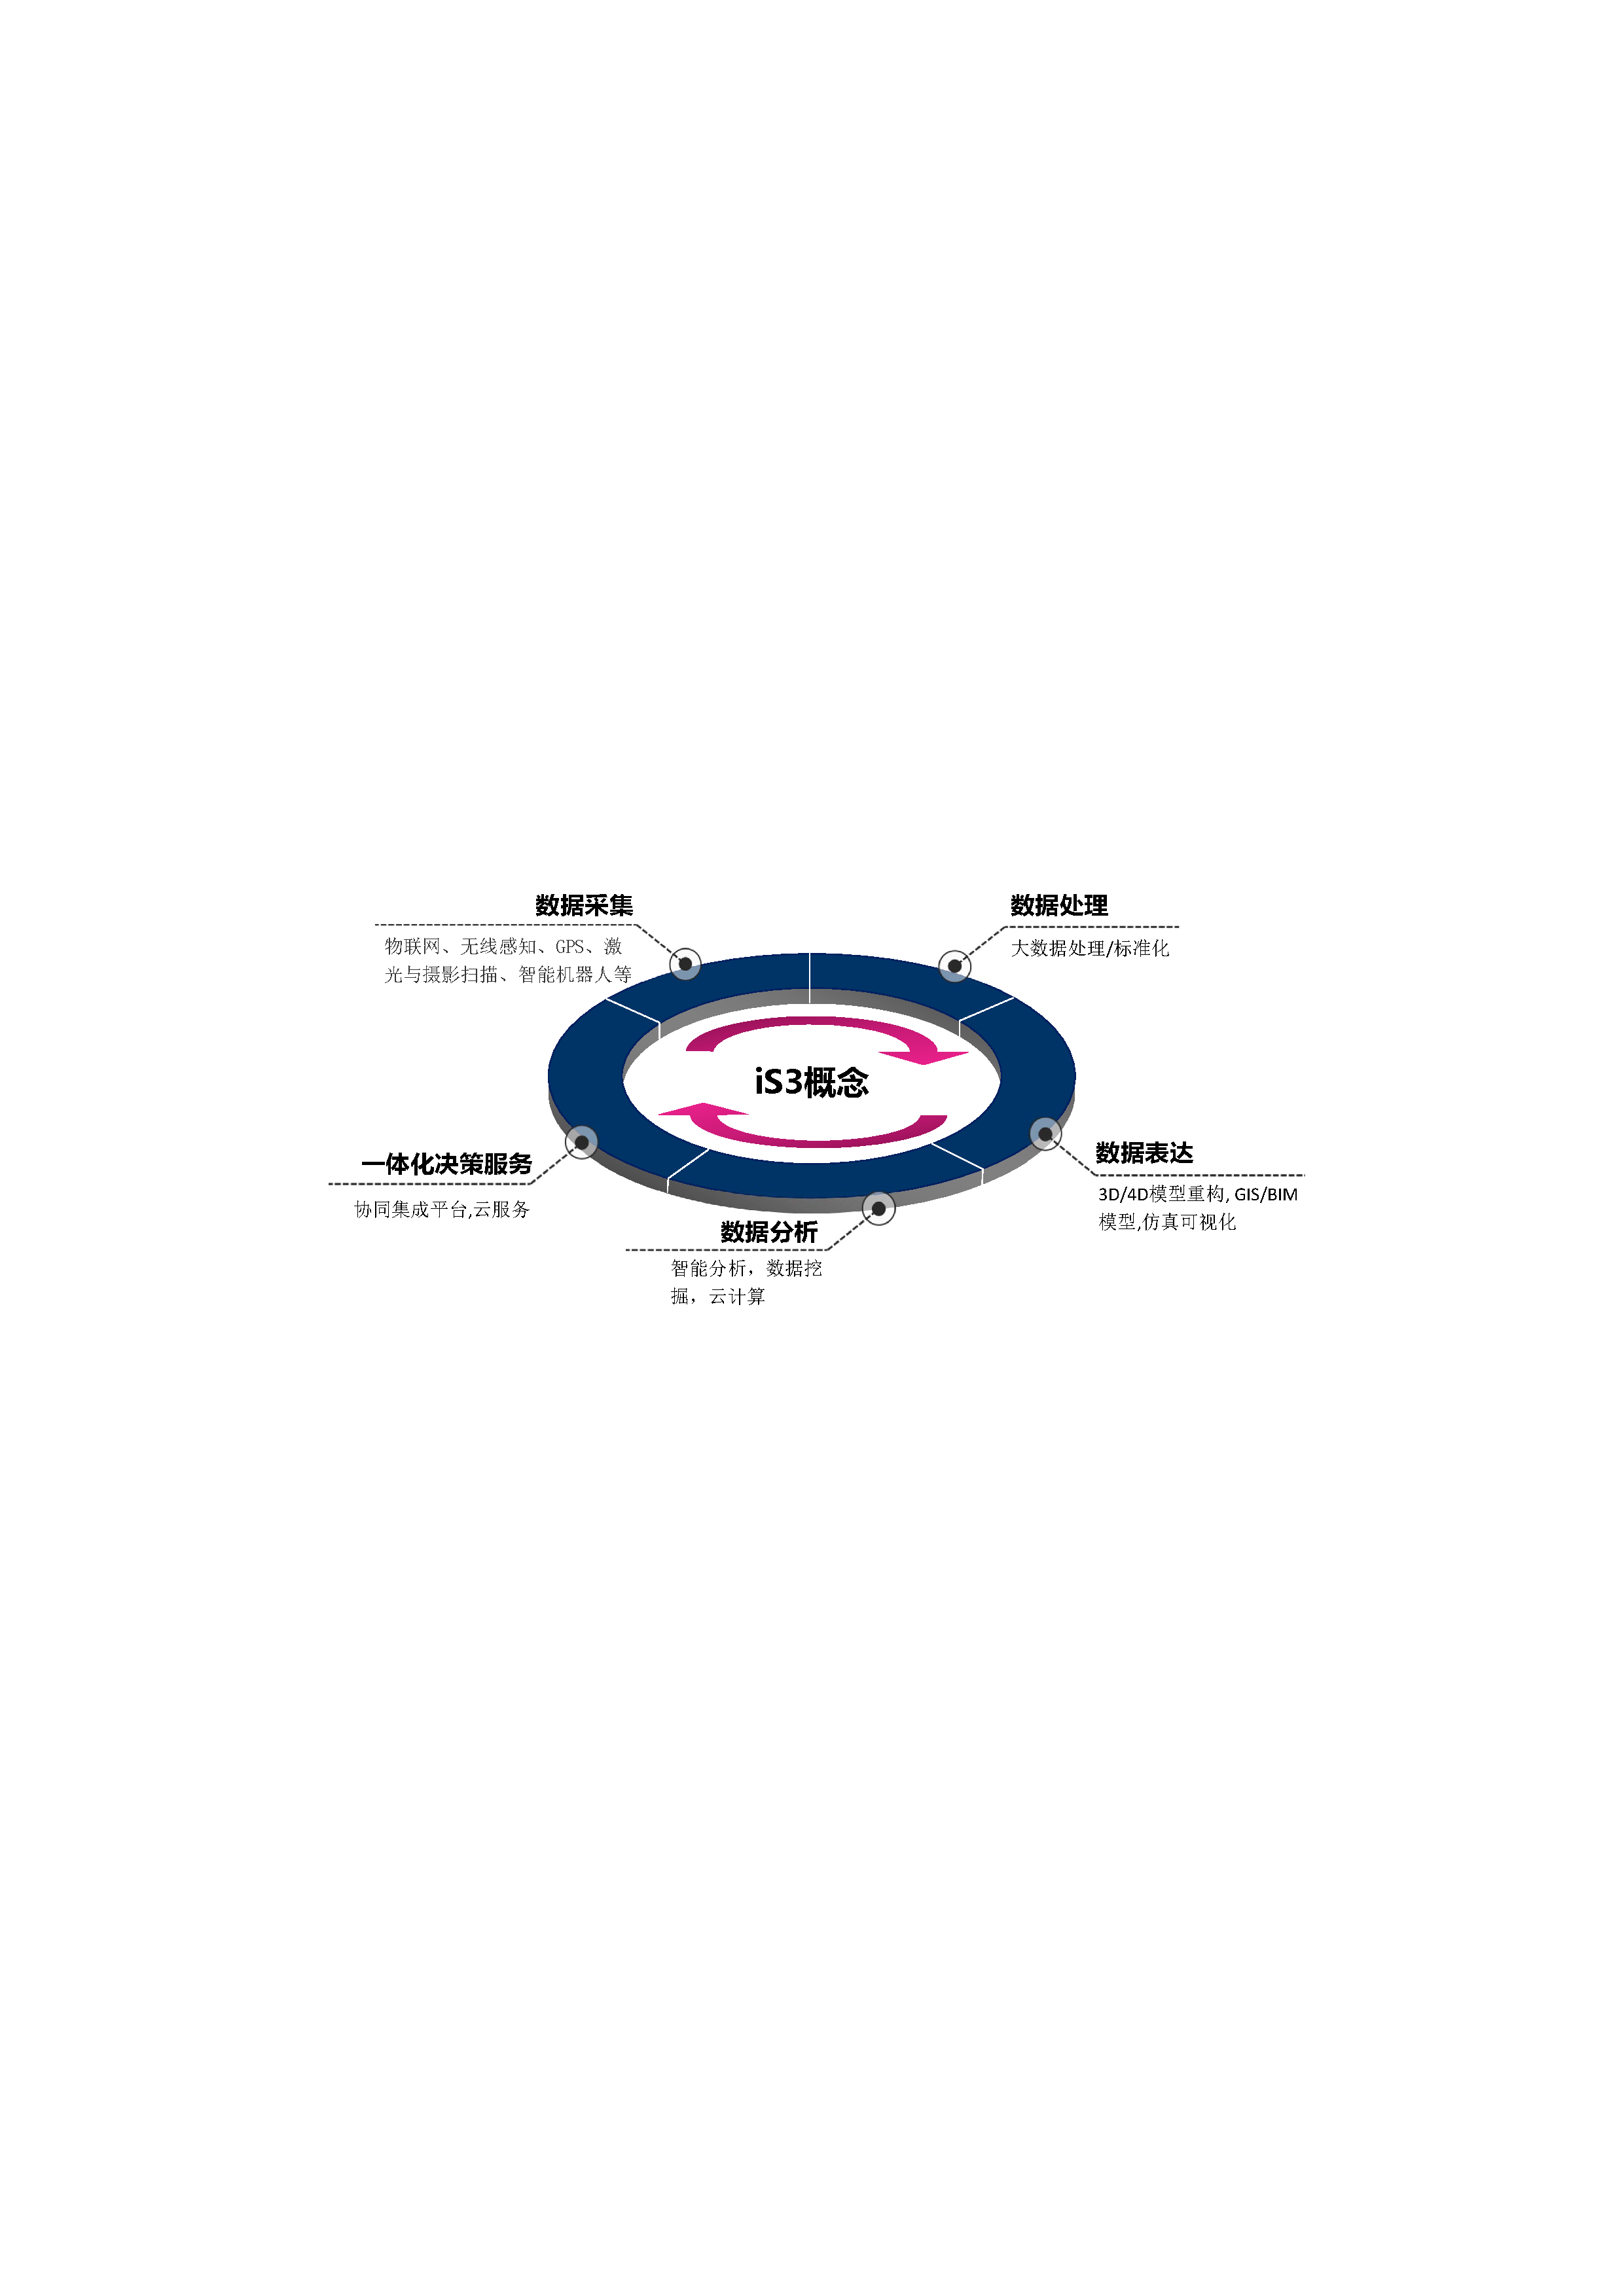
\includegraphics[width=1.0\textwidth]{chap1/iS3.pdf}
	\caption{基础设施智慧服务系统(iS3)概念图(朱合华等,\citeyear{朱合华2018智慧基础设施})}
	\label{fig:iS3概念图}
\end{figure}

%%%%%%%%%%%%%%%%%%%%%%%%%%%%%%%%%%%%%%%%%%%%%%%%%%%%%%%%%%%%%%%%%%%
\section{目前研究存在的问题}

%+++++++++++++++++++++++++++++++++++++++++++++++++++++++++++++++++%
\subsection{服役性能评估的问题}

已有基于单项指标的评估方法未能对盾构隧道的整体服役性能作出评判,而且同一段隧道采用不同的单项指标评估将得到不同的评估结果。目前根据调查研究,盾构隧道在运营期会出现许多病害,如衬砌缺角、掉块、混凝土碳化、剥落、剥离、空洞、钢筋锈蚀、空气水环境中的氯离子、硫酸根离子等(Yuan等,\citeyear{yuan2013predictive})。叶耀东等(\citeyear{叶耀东2007软土地铁运营隧道病害现状及成因分析})总结了上海地铁盾构隧道在运营期的主要病害有渗漏水、裂缝、损坏、纵向沉降和收敛变形等。对于这么多单项病害,现有的单项指标评估方法未对所有的单项指标给出评判标准。不过这种方法因为使用简单,在实际工程应用较多,并编写成行业规范。

已有基于力学模型的评估方法较难建立考虑真实病害情况的数值模型,而且即使有能建立相应的数值模型,其计算分析时间较长。如考虑衬砌纵缝接头的力学性能,建立三维精细化接头力学模型,张厚美等(\citeyear{张厚美2000圆形隧道装配式衬砌接头刚度模型研究})构建的三维有限元模型中,混凝土采用实体单元和弹塑性本构,衬垫采用板单元和曲线本构,连接螺栓采用杆单元,衬垫与混凝土表面之间设置接触单元;曾东洋等(\citeyear{曾东洋2005地铁盾构隧道管片接头刚度影响因素研究})引入面-面接触单元和衬垫单元模拟各构件之间的接触关系;Chen等(\citeyear{chen2009numerical})接头三维精细化有限元模型包括管片、接头、螺栓及手孔等,分析了施工期和服役期盾构隧道管片裂缝或破损问题。虽然上述模型能较好地分析隧道服役性能劣化的原因,但在评估分析过程中比较耗时。

已有基于数学模型的评估方法未考虑各指标之间的相关性和单个指标权重随着指标劣化而变化的情况。在隧道服役性能评估方面,层次分析法因具有综合性强,原理简单等优点,被广泛应用(戴胜,\citeyear{戴胜2008越江盾构隧道耐久性分析与评估体系研究};李晓英等,\citeyear{李晓英2008铁路隧道健康状态模糊评价体系研究};段怀志,\citeyear{段怀志2009隧道及地下工程健康评估研究};张素磊,\citeyear{张素磊2012隧道衬砌结构健康诊断及技术状况评定研究};Rao等,\citeyear{rao2016fuzzy})。根据层次分析法的理论原理(Saaty和Vargas,\citeyear{saaty2012models}),评估指标之间是相互独立的,但实际情况并非如此,如隧道的横向收敛会导致衬砌纵缝的张开量,隧道的纵向变形会导致衬砌环向接缝的张开量和衬砌环错台的发生。另外,由层次分析法评判矩阵计算得出的指标权重是常量,在实际情况中,当某一评估指标劣化严重时,根据“木桶效应”,隧道的整体服役性能应该是迅速下降的,体现为劣化指标权重的增加。

在其他工程领域,已由点状和线状的评估方法向网格化空间评估发展,如洪水灾害评估模型基于空间网格计算洪水灾害损失(Su等,\citeyear{su2005grid});Islam等,\citeyear{islam2007grid};朱强等,\citeyear{朱强2007基于网格的洪水损失计算模型})、铁路轨道网格(或部件)的空间风险评估模型(郭孟欣等,\citeyear{郭孟欣2016基于网格的铁路建设工程风险指数评价模型研究};白磊,\citeyear{白磊2017铁路轨道健康管理网格化分析决策模型研究})、道路工程的网状路面开裂评估模型(Jenelius,\citeyear{jenelius2012road})等,对于盾构隧道相关研究较少。

%+++++++++++++++++++++++++++++++++++++++++++++++++++++++++++++++++%
\subsection{服役性能预测的问题}

盾构隧道服役性能预测缺少既能考虑时间变化趋势,又能考虑数据地理空间关系的预测方法。一般地采用数值模拟结合现场监测数据分析计算盾构隧道的评估指标大小(李喆和张子新,\citeyear{李喆2005相邻隧道施工对上海地铁二号线的影响分析};王如路,\citeyear{王如路2009上海软土地铁隧道变形影响因素及变形特征分析}),大多未研究指标随时间的变化趋势。对于考虑时间因素的数学模型,如马尔科夫链模型(Tran等,\citeyear{tran2008prediction};Abaza和Murad,\citeyear{abaza2009predicting})、时间序列模型(刘燕萍等,\citeyear{刘燕萍2010时间序列分析在建筑物变形监测中的应用};卢宏彬,\citeyear{卢宏彬2016基于时间序列的结构损伤概率方法研究})、BP人工神经网络(Tsuda等,\citeyear{tsuda2006estimating};Mahdevari和Torabi,\citeyear{mahdevari2012prediction})等,均能通过历史数据预测未来某个时间状态的值,但是上述模型只能对同一组数据进行预测,不能考虑空间上临近的数据对该组数据的影响。

%+++++++++++++++++++++++++++++++++++++++++++++++++++++++++++++++++%
\subsection{服役性能服务的问题}

基于地理信息系统的服务平台缺乏对非地理数据的有效管理和用于数据交换、共享、描述工程结构的统一数据标准。GIS系统更像是一个地理数据库的管理系统,且具备十分成熟的拓扑结构,能存储和分析大部分的空间关系,提供了基于矢量和栅格两种方式的空间分析,如图形相交、合并、最短路径、网格计算、面积计算等。

基于建筑信息模型的服务平台缺乏数据信息流管理和开发复杂分析功能的能力。BIM系统注重工程本身在设计、建设时对工程的形状、大小、空间、属性等信息的管理,且提供了便捷、简单的分析功能,如布尔运算、三维造型、碰撞分析、长度面积测量和体积计算等。但是BIM系统的所有功能均需围绕BIM模型展开,对数据全寿命期的数据流动有一定约束,另外BIM采用的直角坐标系统,没有世界地理坐标系统和拓扑结构,在BIM系统中定制复杂的分析功能困难。

考虑上述原因,近些年综合性的智慧服务平台逐渐成为发展趋势,以朱合华等(\citeyear{朱合华2018智慧基础设施})提出的基础设施智慧服务系统(iS3)为例,其从实际工程信息流角度考虑,为服务系统抽象了管理模型、数据模型和分析模型,同时借鉴GIS和BIM系统的数据存储、管理和分析功能,为工程数据和图形引擎提供开放式的接口,实现各类分析和智慧决策的服务,如图~\ref{fig:iS3-gis-bim}~所示。

目前此类综合性平台基本采用单体式应用的方式进行开发,尽管其在开发过程中是模块化的逻辑,但最终会被发布成单个应用,如C++、C\#的EXE格式,Java的WAR格式,这种方式有很大的局限性,随着时间推移,应用会越来越庞大,越难理解,不利于持续性开发,另外单体式应用某个模块的一个问题有可能导致整个系统奔溃。故现有的服务平台缺少一种低耦合、高可靠、易扩展的服务框架。

\begin{figure}[!h]
	\centering
	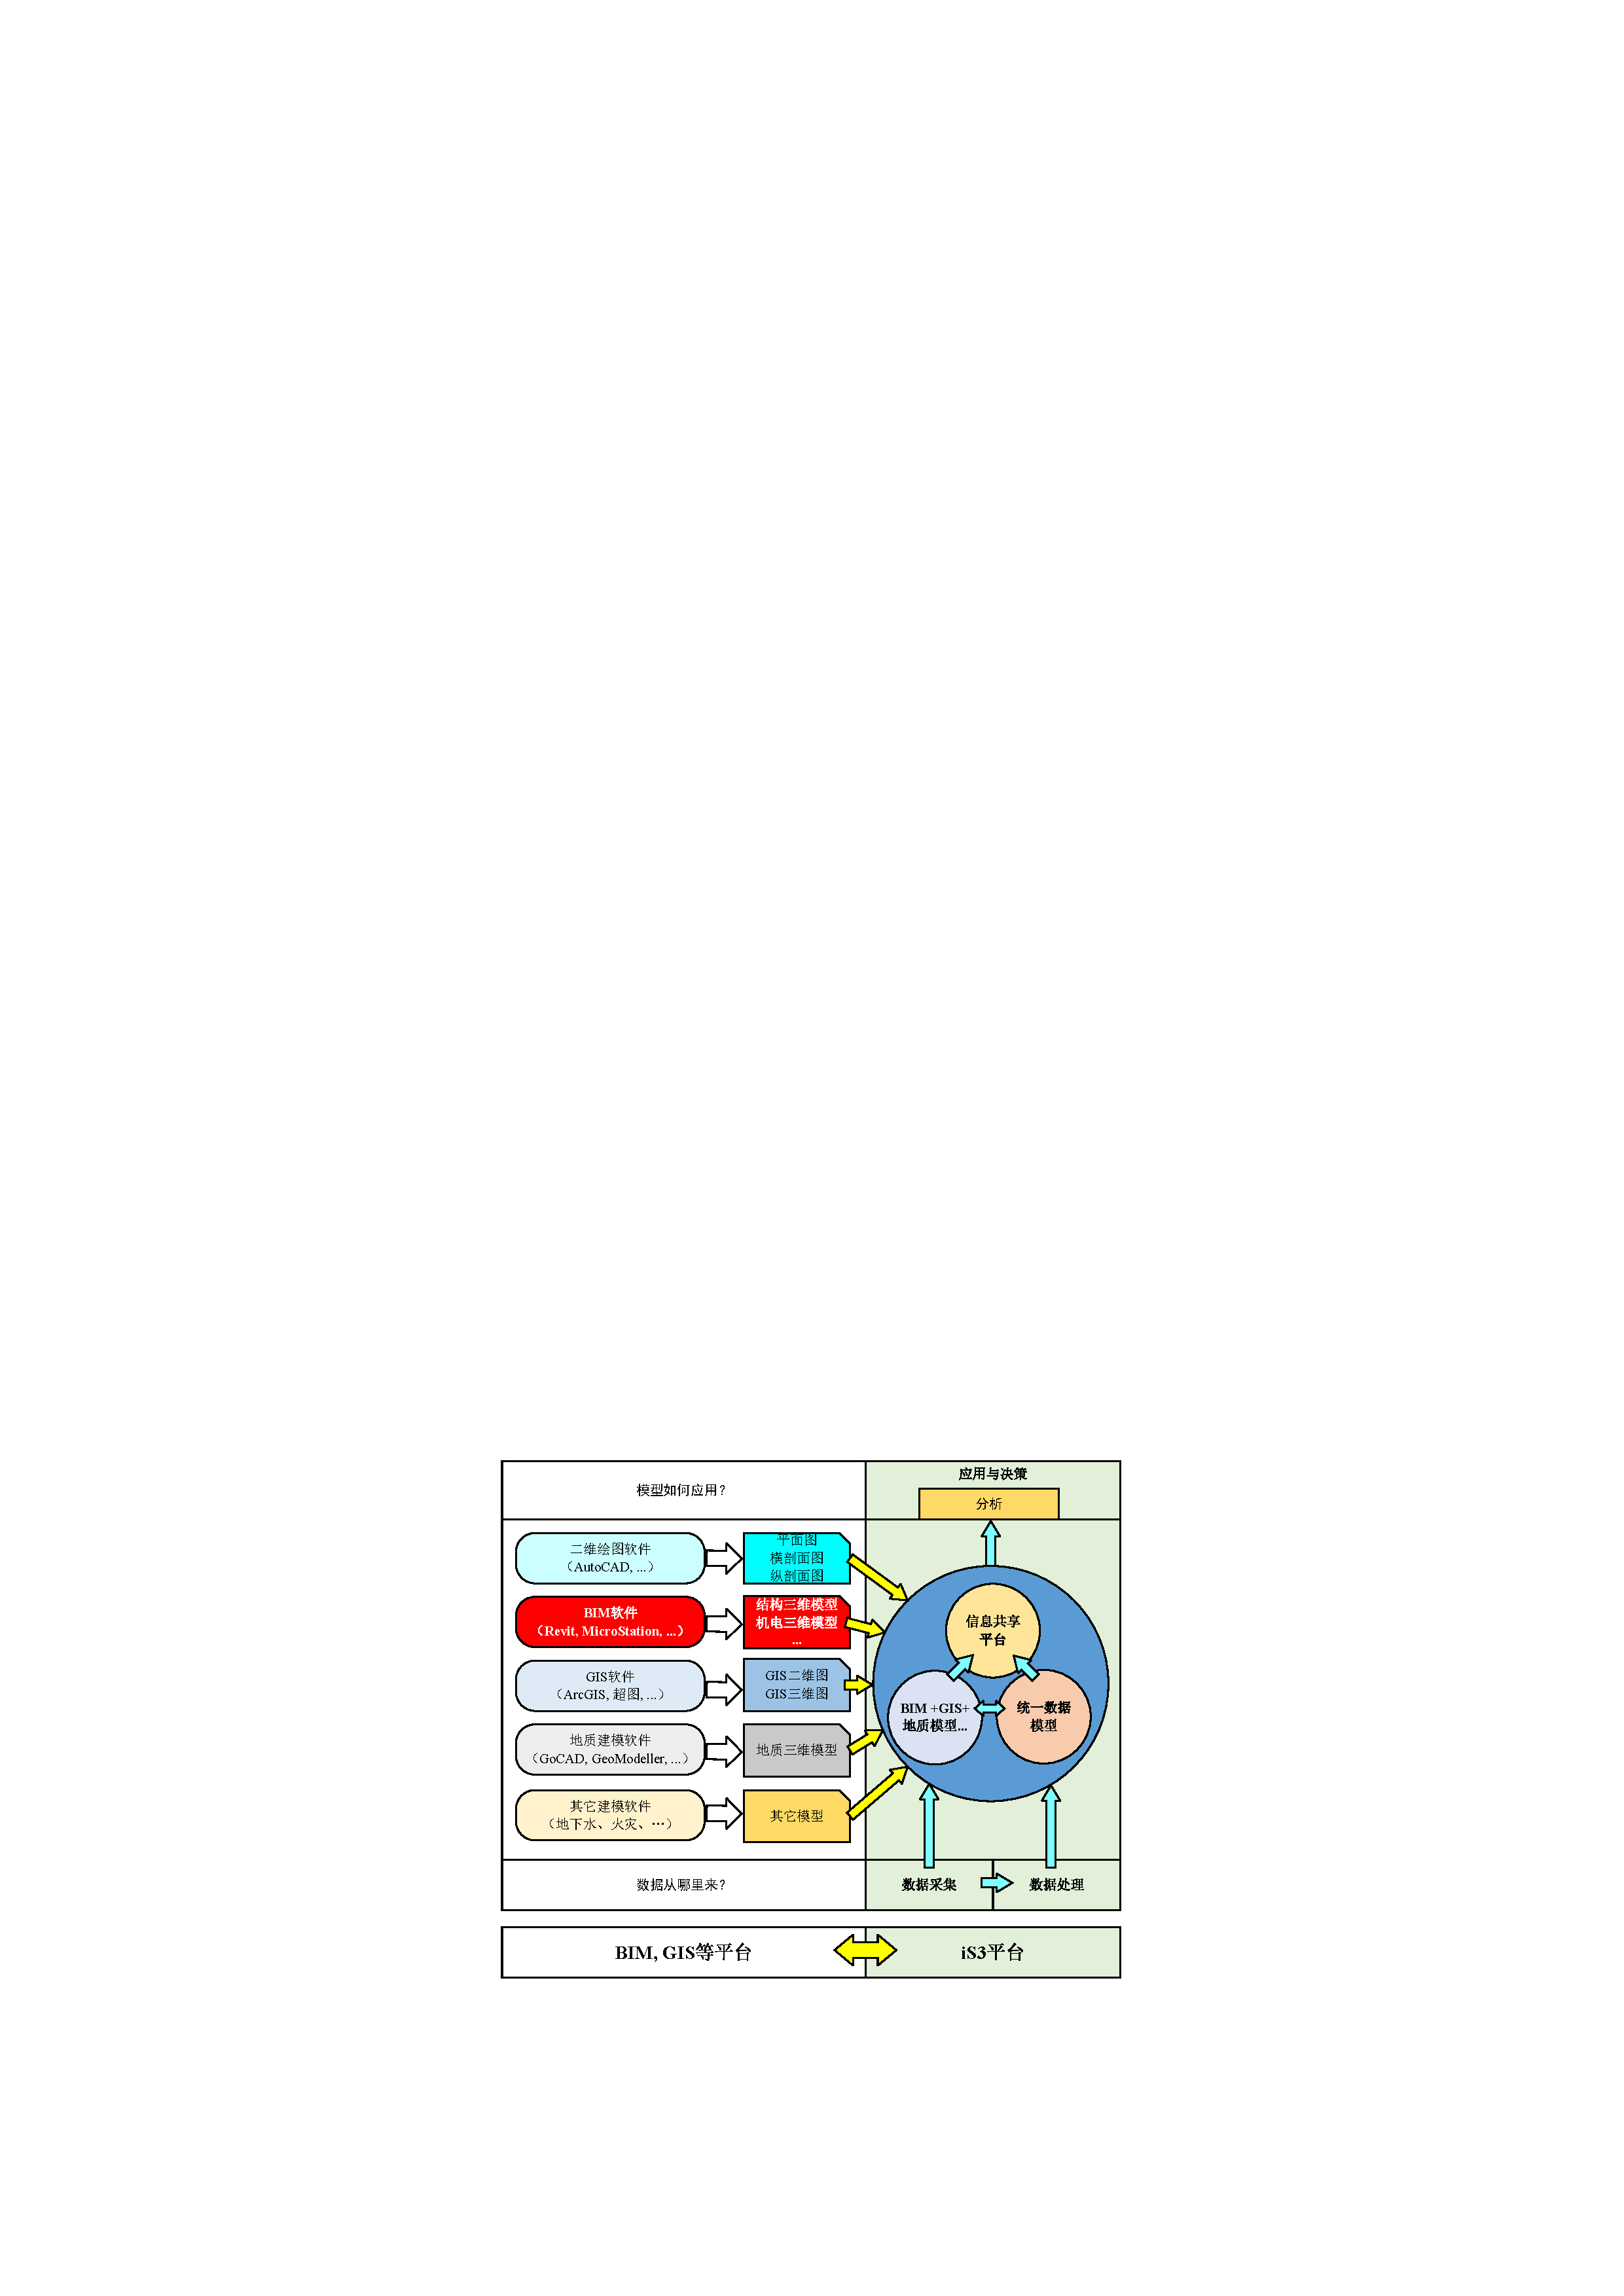
\includegraphics[width=0.9\textwidth]{chap1/iS3-gis-bim.pdf}
	\caption{iS3 与 BIM, GIS 的区别与联系}
	\label{fig:iS3-gis-bim}
\end{figure}

%%%%%%%%%%%%%%%%%%%%%%%%%%%%%%%%%%%%%%%%%%%%%%%%%%%%%%%%%%%%%%%%%%%
\section{论文研究内容、路线和创新点}

%+++++++++++++++++++++++++++++++++++++++++++++++++++++++++++++++++%
\subsection{主要研究内容}

本文以上海运营地铁盾构隧道为研究对象,研究如何根据已有的监测检测数据,客观定量地评估盾构隧道当前服役性能,且在大量历史数据基础上,对未来某个时间盾构隧道的服役性能作出预测,以及探讨了服役性能评估与预测方法在实际工程中的服务机制。各章节的主要研究内容如下:

第二章参考美国国家公路协会对路面服役性能评估方法,对盾构隧道进行病
害数据采集,专家打分,和打分结果的回归拟合,得出适合盾构隧道的服役性能指标,建立服役性能指标与相对沉降平均值${sett}_{a}$、平均差异沉降$set{{t}_{d\_a}}$、平均收敛变形率${cov}_{a}$、百环渗漏水面积${d}_{l}$、百环衬砌剥落面积${d}_{s}$、百环裂缝长度${d}_{c}$的定量公式,并采用变权理论对公式进行全寿命期的修正。

第三章研究了适用于盾构隧道沉降预测的自回归滑动平均模型和结构向量时间序列模型,考虑了不同沉降时间序列之间的空间关联性,提供对历史沉降数据的拟合以及未来沉降数据的预测精度,利用单一沉降数据的预测,得出服役性能指标的退化曲线。

第四章采用微服务架构改进传统的单体式应用模块复杂、体量庞大、可扩展性差的问题,研究了盾构隧道服役性能相关的数据服务、服役性能分析服务和有限元分析服务的微服务架构关键技术,包括服务接口标准和网关设计、微服务间的通信模式,服务的管理与发现机制。

第五章以上海地铁盾构隧道为工程依托,介绍了基础设施智慧服务系统(iS3)以及盾构隧道服役性能评估与预测的微服务体系,并在iS3平台上集成微服务架构体系,实现分析功能即服务的概念。

第六章总结了本文的主要研究成果以及相应的结论,并对以后的研究工作提出了展望。 

%+++++++++++++++++++++++++++++++++++++++++++++++++++++++++++++++++%
\subsection{技术路线}

本文技术路线如图~\ref{fig:本文技术路线}~所示。

\begin{figure}[htb!]
    \centering
    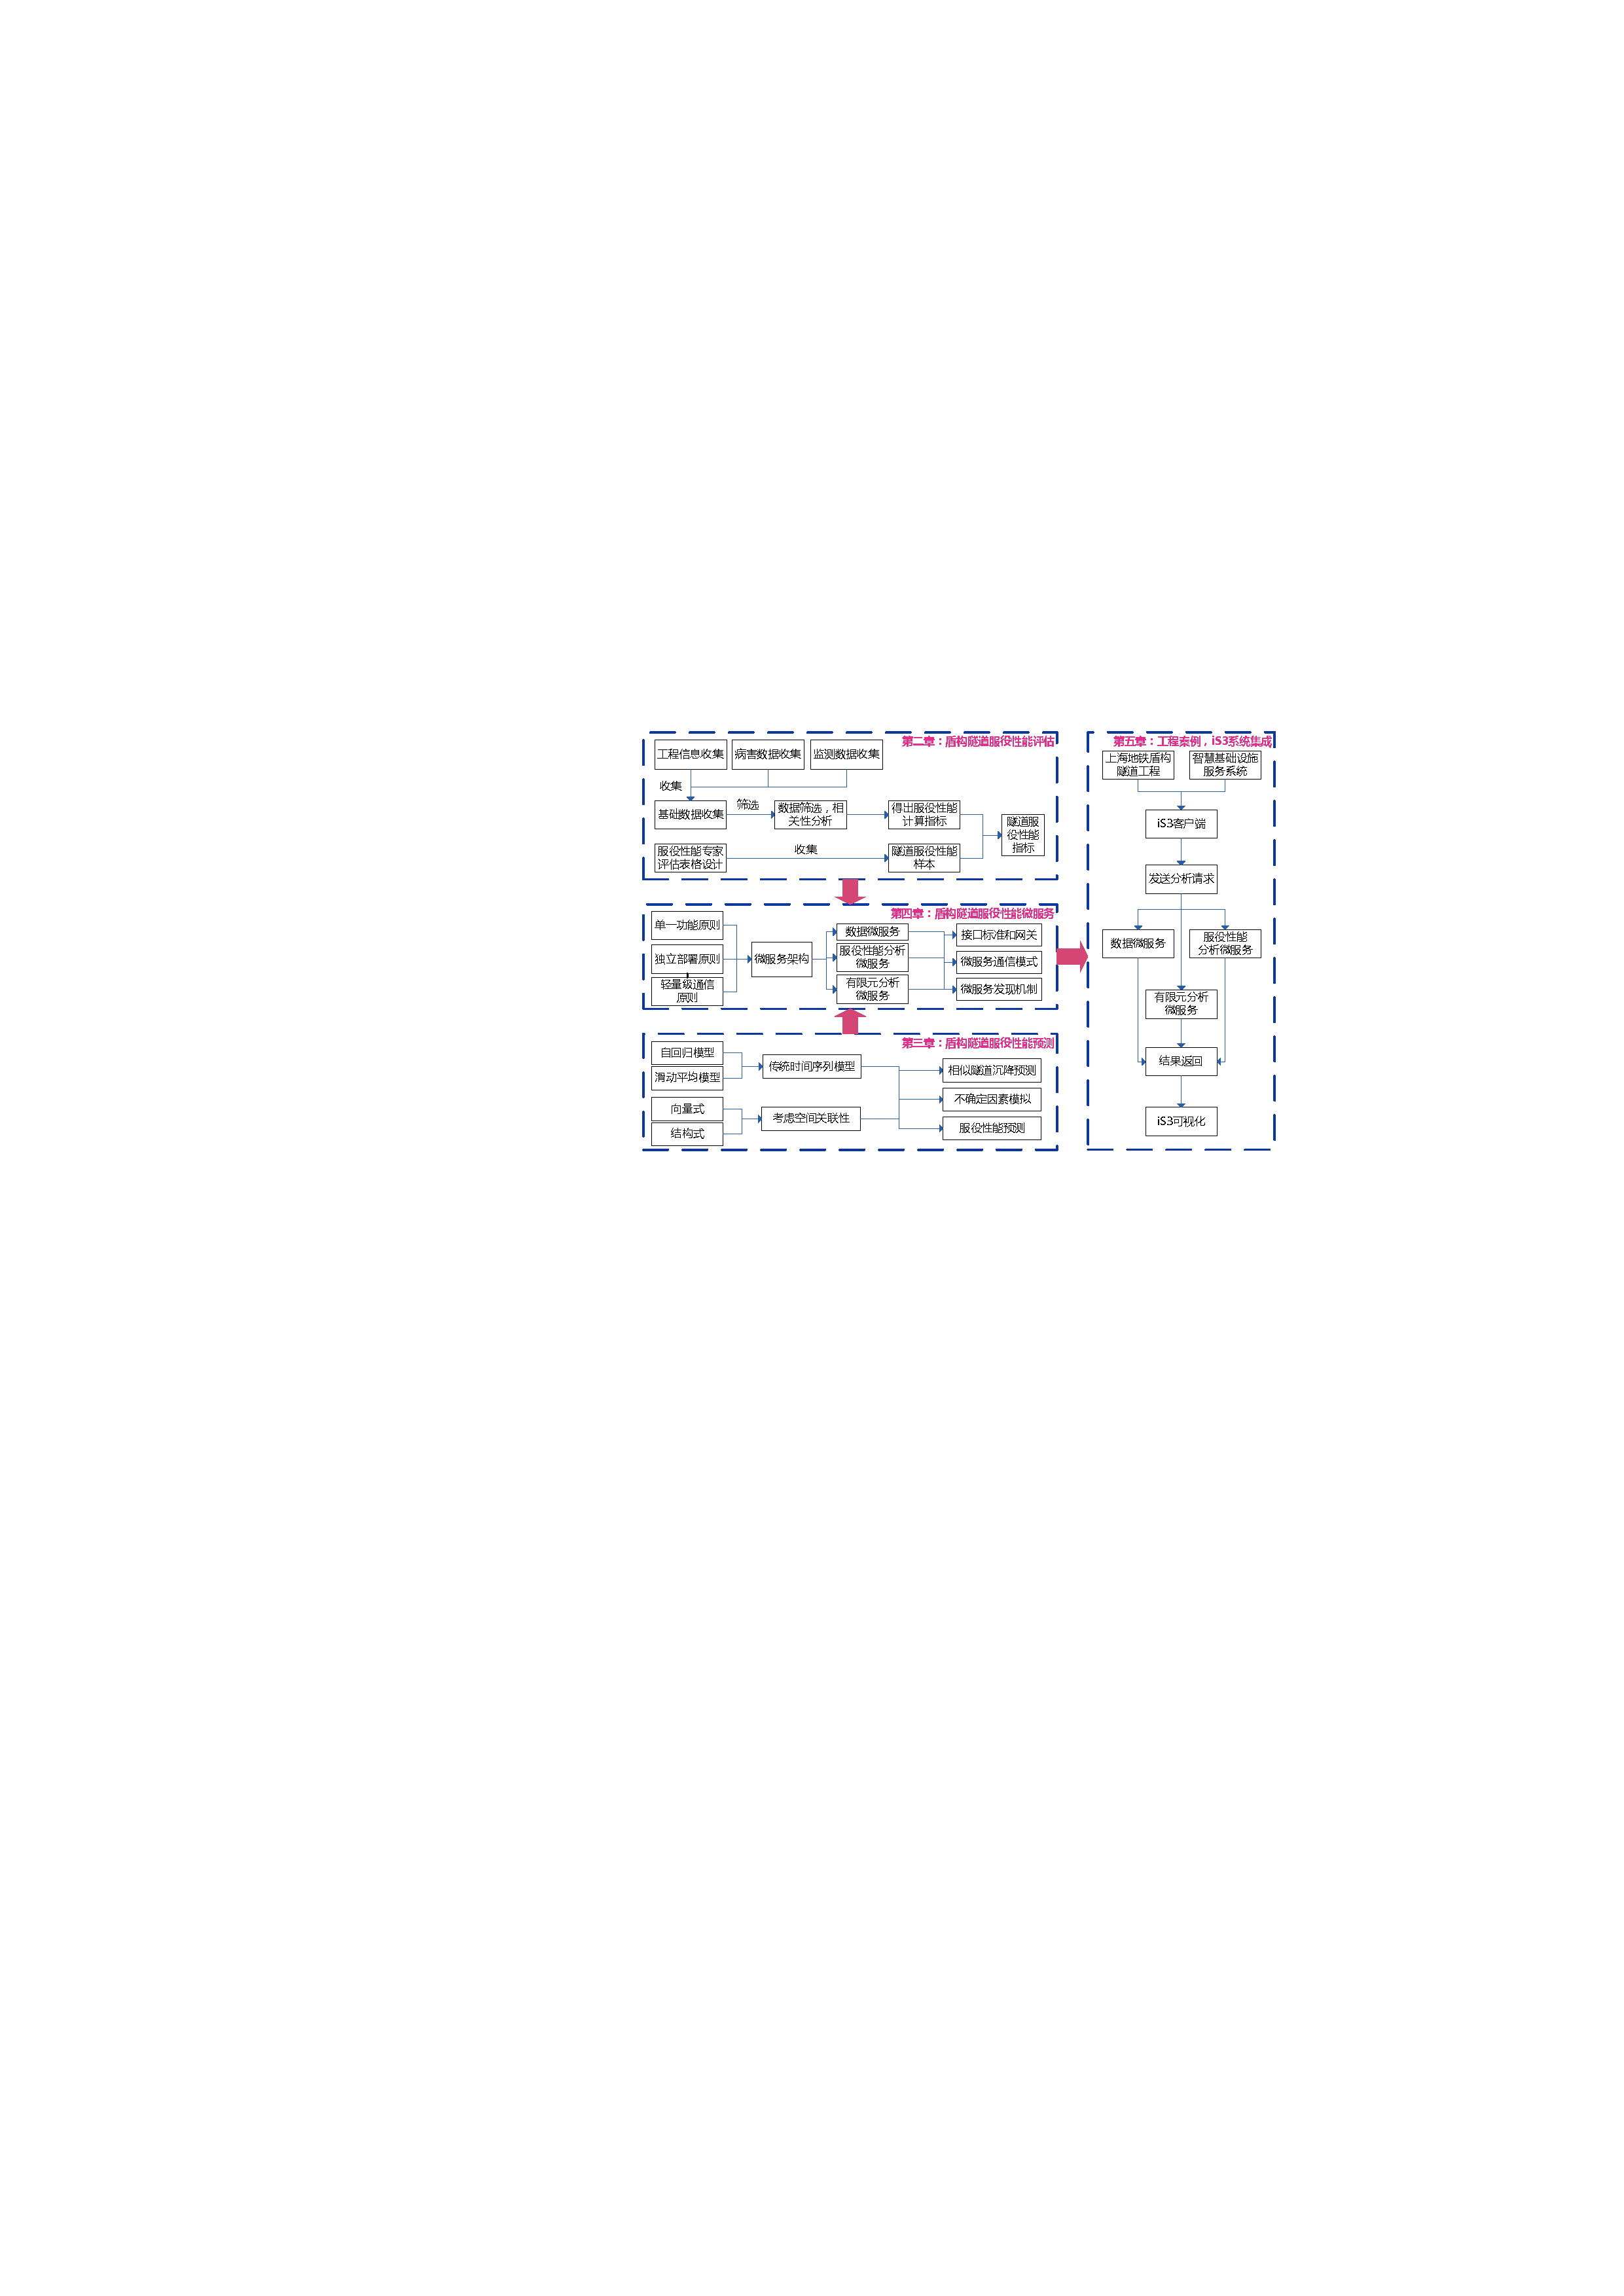
\includegraphics[width=1.0\textwidth]{chap1/process.pdf}
    \caption{本文技术路线}
    \label{fig:本文技术路线}
\end{figure}

%+++++++++++++++++++++++++++++++++++++++++++++++++++++++++++++++++%
\subsection{主要创新点}

本文主要创新点有:

(1)提出定量化盾构隧道服役性能指标(TSI)计算公式,并应用于宏观空间网格化评估。

(2)建立考虑同期沉降空间关联性的结构-向量时间序列模型,由此得出服役性能指标的退化模型。

(3)研究和设计了盾构隧道服役性能相关分析功能的分布式微服务框架,具备可扩展性强、独立开发部署和分析功能即服务等优点。